\section{Perancangan Sistem}

Berdasarkan hasil analisis sistem dan wawancara dengan pihak terkait, sistem dirancang untuk mendigitalkan proses pencatatan yang sebelumnya manual dan belum terintegrasi, sekaligus untuk mendeteksi penyewa yang berpotensi melakukan pelanggaran. Pendekatan ini berfokus pada integritas data, keamanan akses, dan kemudahan pemantauan melalui notifikasi jika data yang diinput merupakan penyewa yang berpotensi melakukan pelanggaran.

Informasi yang diperoleh melalui observasi lapangan, studi dokumentasi, serta wawancara dengan pengelola apartemen menjadi masukan penting dalam penyusunan arsitektur sistem. Misalnya, saat Pelaku Komersil hendak mendaftar harus input NIB (Nomor Induk Berusaha) agar jika suatu saat Pelaku Komersil melakukan pelanggaran akan lebih mudah untuk diproses hukum. Selain itu, sistem perlu memperhatikan bahwa pola penyewaan jangka pendek seperti harian atau mingguan dapat berbeda secara perilaku dari penyewaan bulanan. Oleh karena itu, sistem dikembangkan dengan mempertimbangkan fleksibilitas input jenis sewa. Selain pencatatan data utama, sistem juga mencatat seluruh aktivitas perubahan data yang dilakukan oleh Pelaku Komersil dalam bentuk \textit{log history}, sebagai jejak digital yang bisa digunakan untuk audit atau konfirmasi jika terjadi ketidaksesuaian data.

\newpage
\subsection{Arsitektur Sistem}
Sejalan dengan landasan teori mengenai teknologi web yang telah diuraikan pada Bab~\ref{chap:teori}, sistem \textit{data capture} ini dibangun menggunakan arsitektur \textit{client-server}. Spesifikasi teknis dari komponen arsitektur tersebut disesuaikan dengan kebutuhan integrasi dan efisiensi sistem sebagai berikut.

\begin{itemize}
    \item \textbf{Antarmuka Pengguna (\textit{Frontend}):} Dibangun menggunakan pustaka \textbf{React.js} bersama perkakas \textit{build} \textbf{Vite} untuk menghasilkan antarmuka web yang interaktif (\textit{Single Page Application}) bagi Pelaku Komersil dan Pengelola. Komunikasi pertukaran data ke peladen (\textit{server}) ditangani menggunakan \textbf{Axios}.
    \item \textbf{Sistem \textit{Backend}:} Menggunakan lingkungan eksekusi \textbf{Node.js} dengan kerangka kerja (\textit{framework}) \textbf{Express.js} untuk menangani pemrosesan logika bisnis serta menyediakan layanan \textit{RESTful API} secara asinkronus.
    \item \textbf{Basis Data:} Menggunakan \textbf{MySQL} yang terpusat dengan ekosistem utama SRusun untuk penyimpanan data relasional. Akses menuju basis data dioptimalkan menggunakan pustaka \texttt{mysql2/promise} melalui mekanisme \textit{connection pooling} agar tangguh dalam menangani koneksi konkuren.
    \item \textbf{Manajemen Berkas:} Pustaka \textit{middleware} \textbf{Multer} digunakan untuk menangani pengiriman formulir \textit{multipart/form-data}, yang memfasilitasi proses pengunggahan (\textit{upload}) dokumen bukti pelanggaran yang disimpan secara aman pada peladen.
    \item \textbf{Keamanan dan Autentikasi:} 
    \begin{itemize}
        \item Autentikasi pengguna difasilitasi oleh mekanisme \textit{Single Sign-On} (SSO), sehingga sistem tidak lagi mewajibkan penyimpanan kata sandi mandiri maupun manajemen sesi lokal berskala kecil.
        \item Verifikasi hak akses menggunakan \textbf{JSON Web Token (\textit{JWT})} dari ekosistem SRusun (melalui modul \texttt{jsonwebtoken}) guna menjamin proses otorisasi secara terpusat dan aman.
        \item Modul \textbf{CORS} (\textit{Cross-Origin Resource Sharing}) diterapkan pada \textit{middleware} peladen untuk menjaga keamanan terhadap interaksi lintas domain yang tidak berwenang.
    \end{itemize}
    \item \textbf{Ekspor Data:} Fitur konversi kumpulan data internal ke struktur format \textbf{CSV} didukung oleh pustaka \textbf{json2csv} untuk memenuhi kebutuhan \textit{audit trail} (\textit{log} aktivitas) dan pelaporan eksternal kepada pihak Pengelola.
    \item \textbf{Deployment:} Digunakan \textit{process manager} \textbf{PM2} untuk mengelola aplikasi agar tetap siaga di latar belakang (\textit{daemon}) didampingi oleh \textbf{NGINX} sebagai \textit{reverse proxy} untuk mendistribusikan lalu lintas jaringan.
\end{itemize}

% \subsection{Pemodelan Sistem}
% Disusunlah alur sistem deteksi penyewa mencurigakan dalam bentuk beberapa diagram visual, seperti {flowchart}, {use case diagram}, ERD, dan diagram basis data. Diagram-diagram ini bertujuan untuk menjelaskan proses dari awal pengumpulan data penyewa (\textit{data capture}) hingga tahapan analisis dan pemberian notifikasi apabila ditemukan penyewa dengan aktivitas mencurigakan. 

% \begin{figure}[H]
%     \centering
%     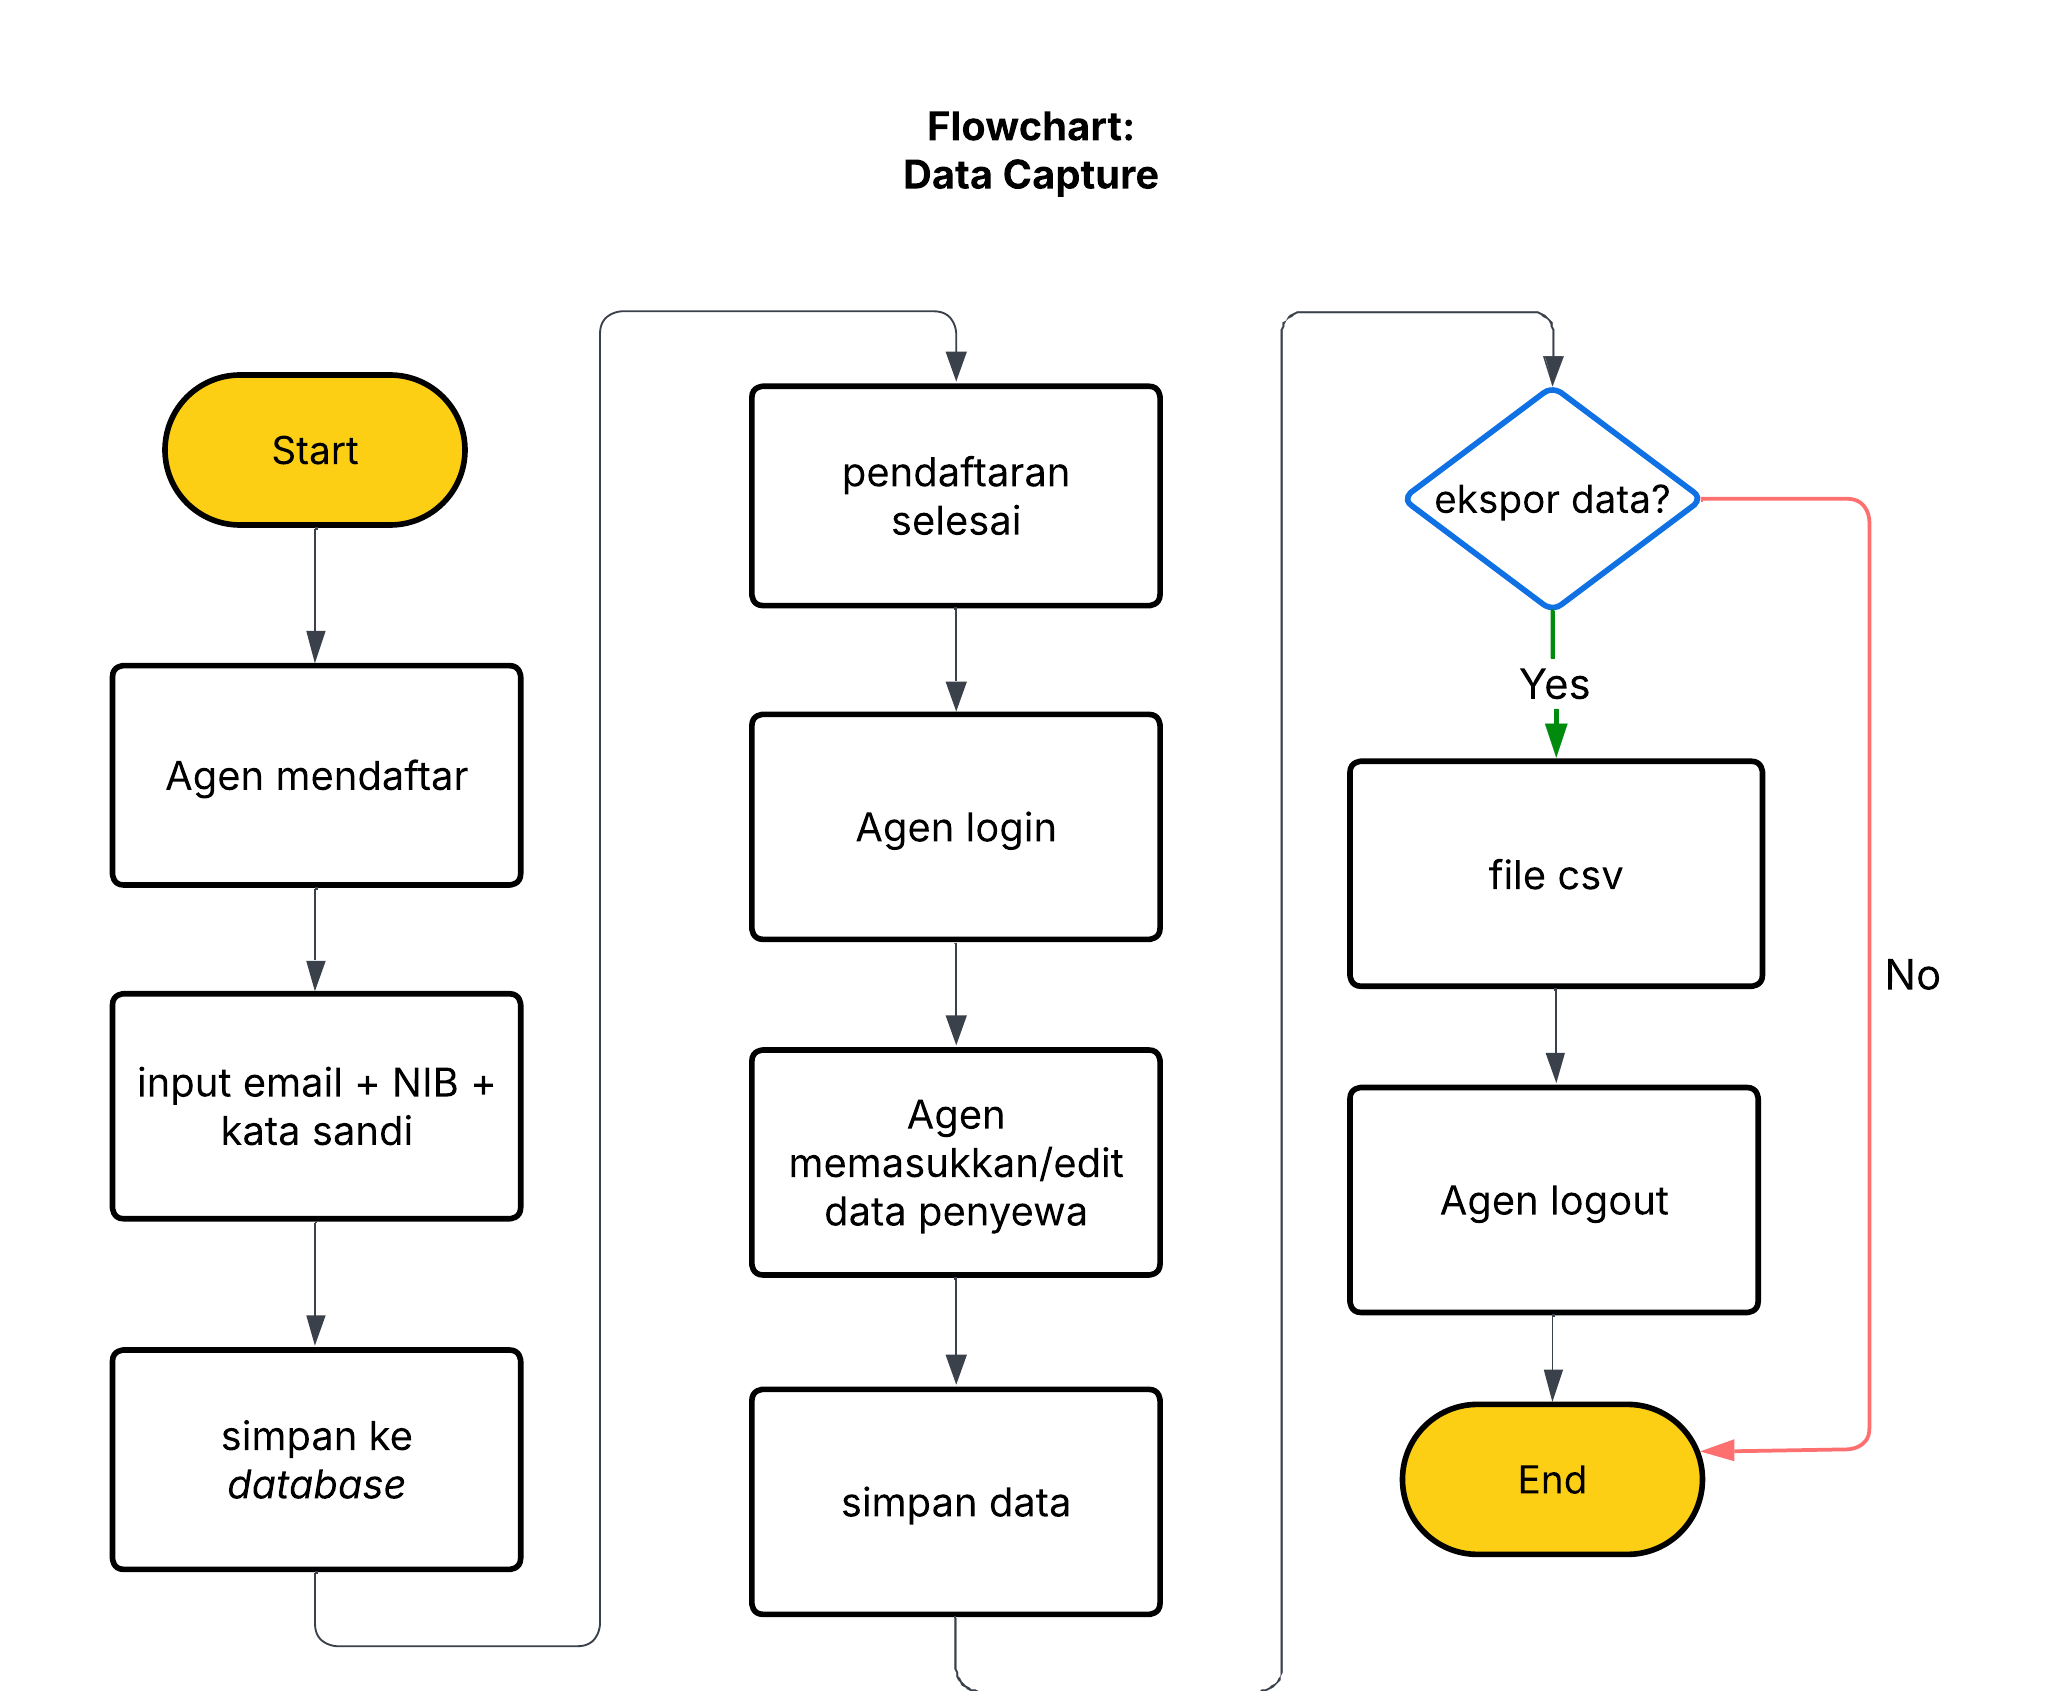
\includegraphics[width=0.7\textwidth]{Gambar/Flowchart Sistem Data Capture.png}
%     \caption{Flowchart untuk Sistem \textit{Data Capture}}
%     \label{fig:flowchart_data_capture}
% \end{figure}

% \newpage
% Gambar~\ref{fig:flowchart_data_capture} menjelaskan alur sistem dari pendaftaran Pelaku Komersil, input data penyewa, hingga penyimpanan data ke basis data. Sistem juga memfasilitasi ekspor data dalam format CSV, serta menyediakan fitur \textit{log} perubahan data.

% \begin{figure}[H]
%     \centering
%     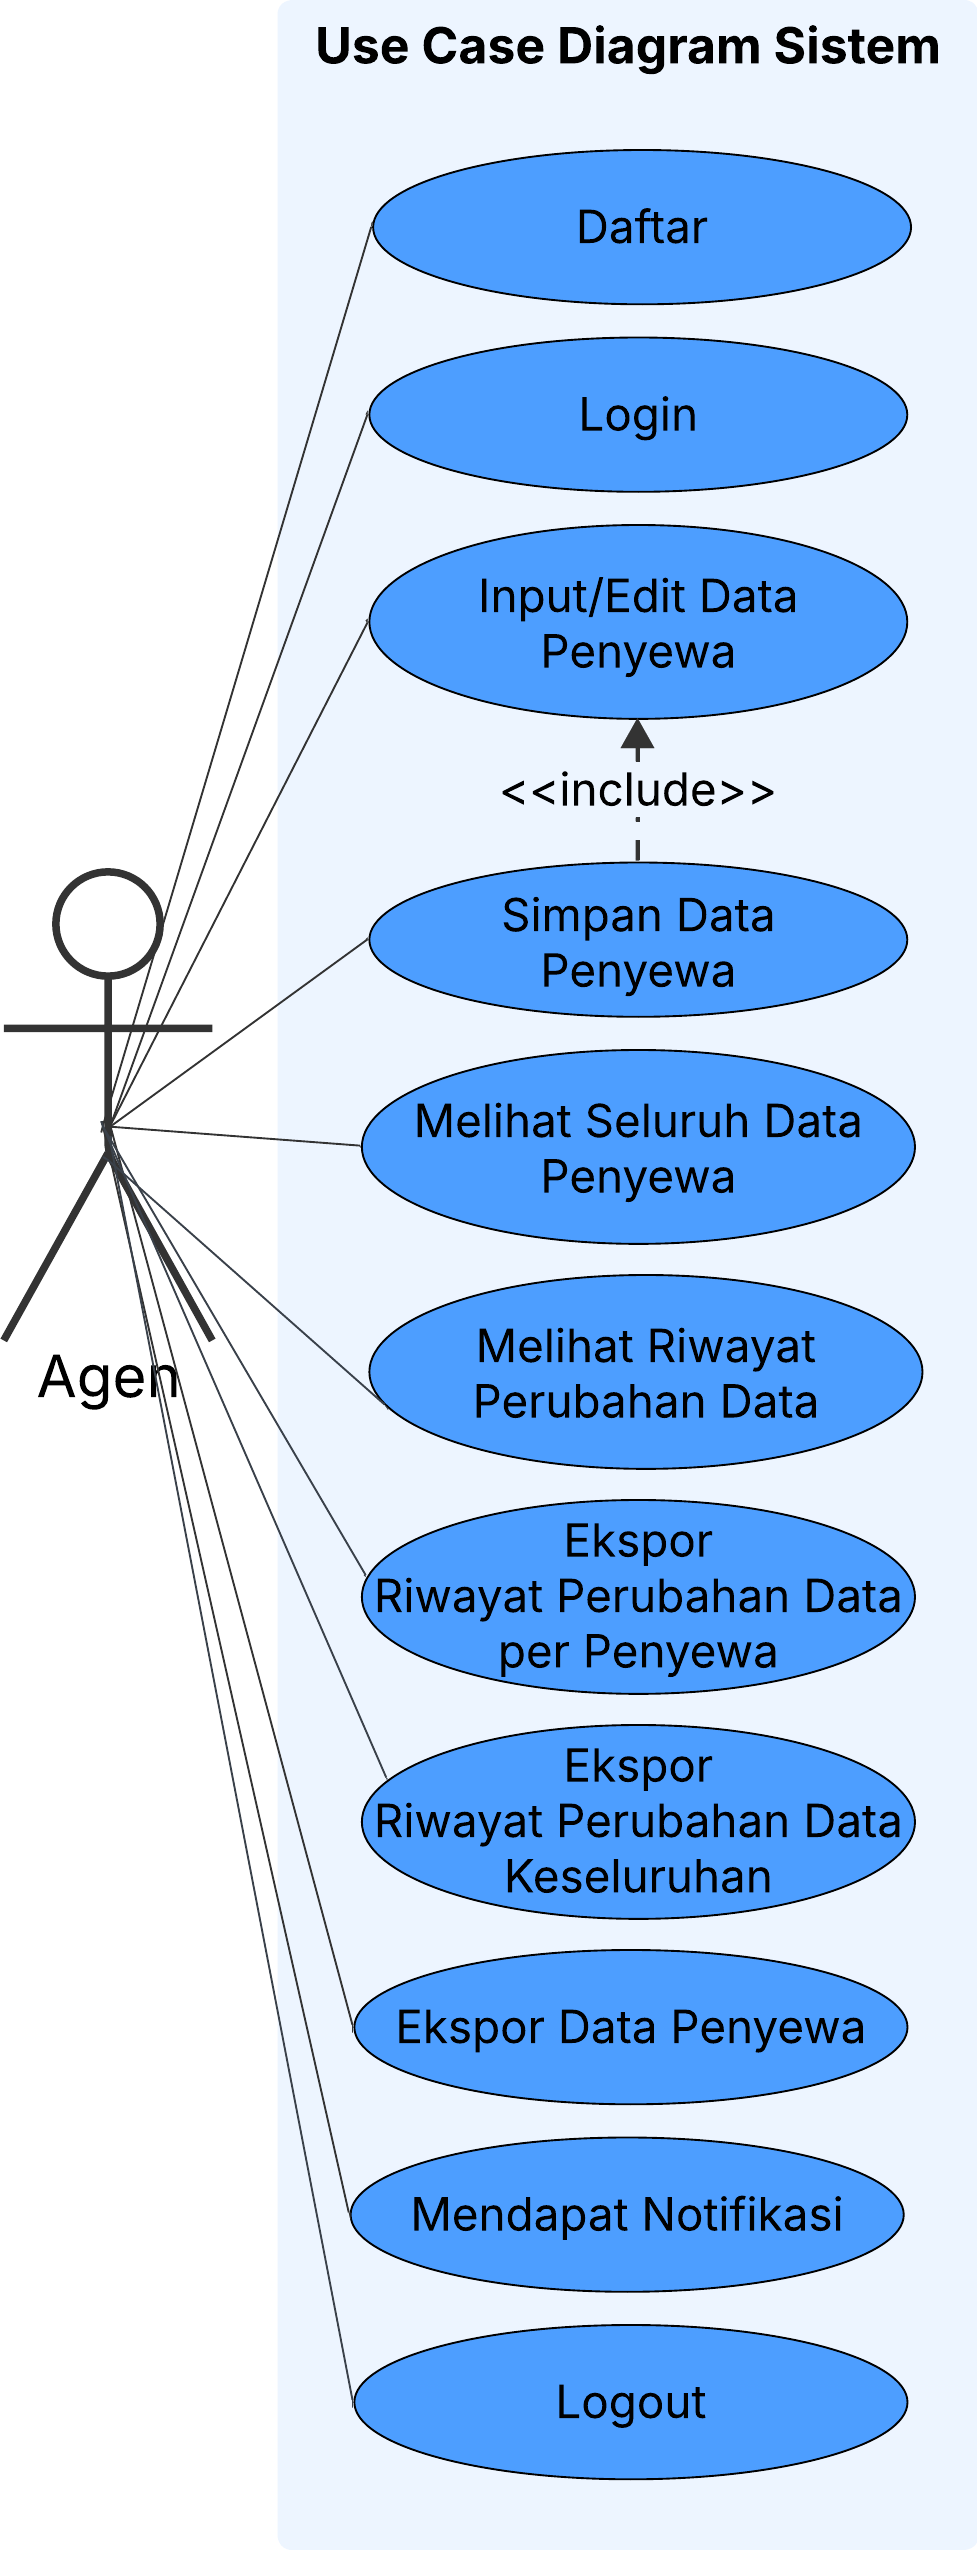
\includegraphics[width=0.47\textwidth, height=0.6\textheight, keepaspectratio]{Gambar/Use Case Diagram System.png}
%     \caption{\textit{Use Case Diagram} Sistem}
%     \label{fig:use_case_data_capture}
% \end{figure}

% Gambar~\ref{fig:use_case_data_capture} menjelaskan interaksi antara Pelaku Komersil dan Pengelola dengan fitur-fitur dalam sistem.

% \begin{figure}[H]
%     \centering
%     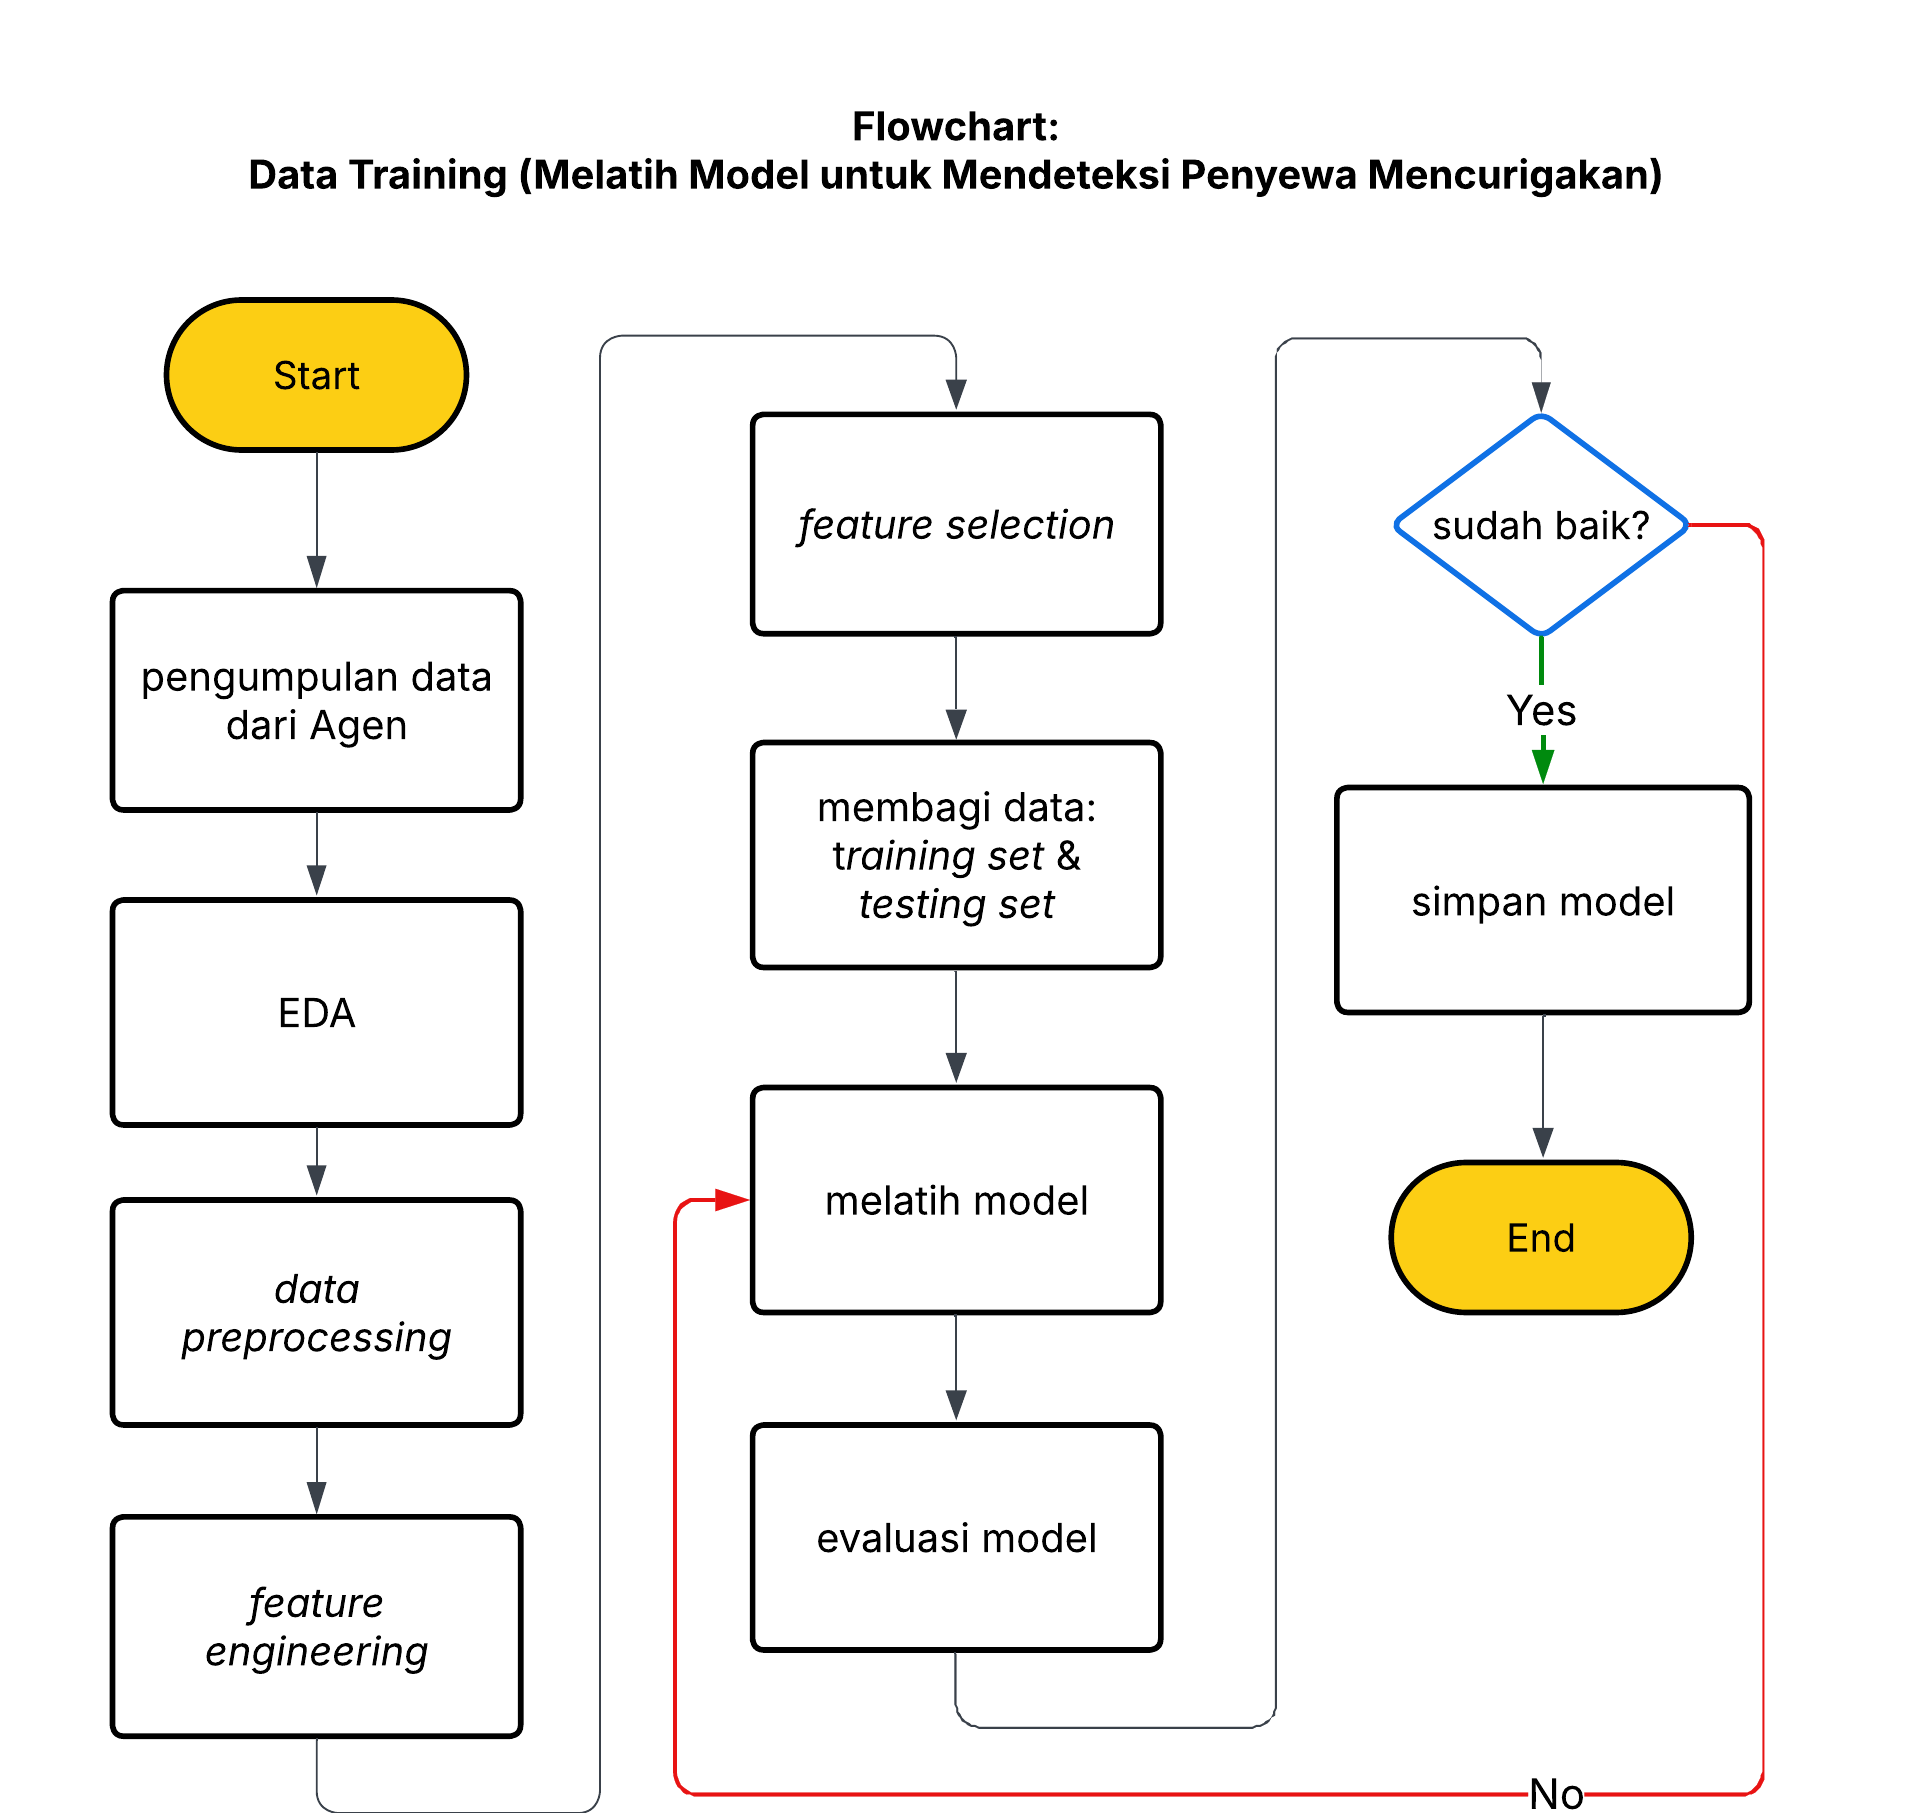
\includegraphics[width=0.7\textwidth]{Gambar/Flowchart Proses Data Training.png}
%     \caption{Flowchart \textit{Data Training}}
%     \label{fig:flowchart_data_training}
% \end{figure}

% Gambar~\ref{fig:flowchart_data_training} menunjukkan proses persiapan data historis penyewa yang akan digunakan sebagai data pelatihan (\textit{training data}) untuk model klasifikasi. Data pelatihan ini menjadi fondasi dalam mengenali pola perilaku penyewa.

% \begin{figure}[H]
%     \centering
%     
\includegraphics[width=0.7\textwidth]{Gambar/Flowchart Proses Analisis & Notif.png}
%     \caption{Flowchart untuk Deteksi Penyewa Mencurigakan}
%     \label{fig:flowchart_deteksi_penyewa_mencurigakan}
% \end{figure}

% Gambar~\ref{fig:flowchart_deteksi_penyewa_mencurigakan} menggambarkan bagaimana data yang sudah dikumpulkan dianalisis dan diverifikasi. Jika ditemukan pola atau parameter yang mencurigakan (misalnya metode pembayaran tertentu yang tidak biasa, waktu \textit{check-in} di luar jam normal, atau lama tinggal yang tidak sesuai jenis sewa), maka sistem dapat memberikan peringatan atau notifikasi.

% Hubungan antar entitas data utama (Users, Rentals, Units, Violations, dan Rental Logs) dimodelkan dalam diagram hubungan entitas berikut:

% \begin{figure}[H]
%     \centering
%     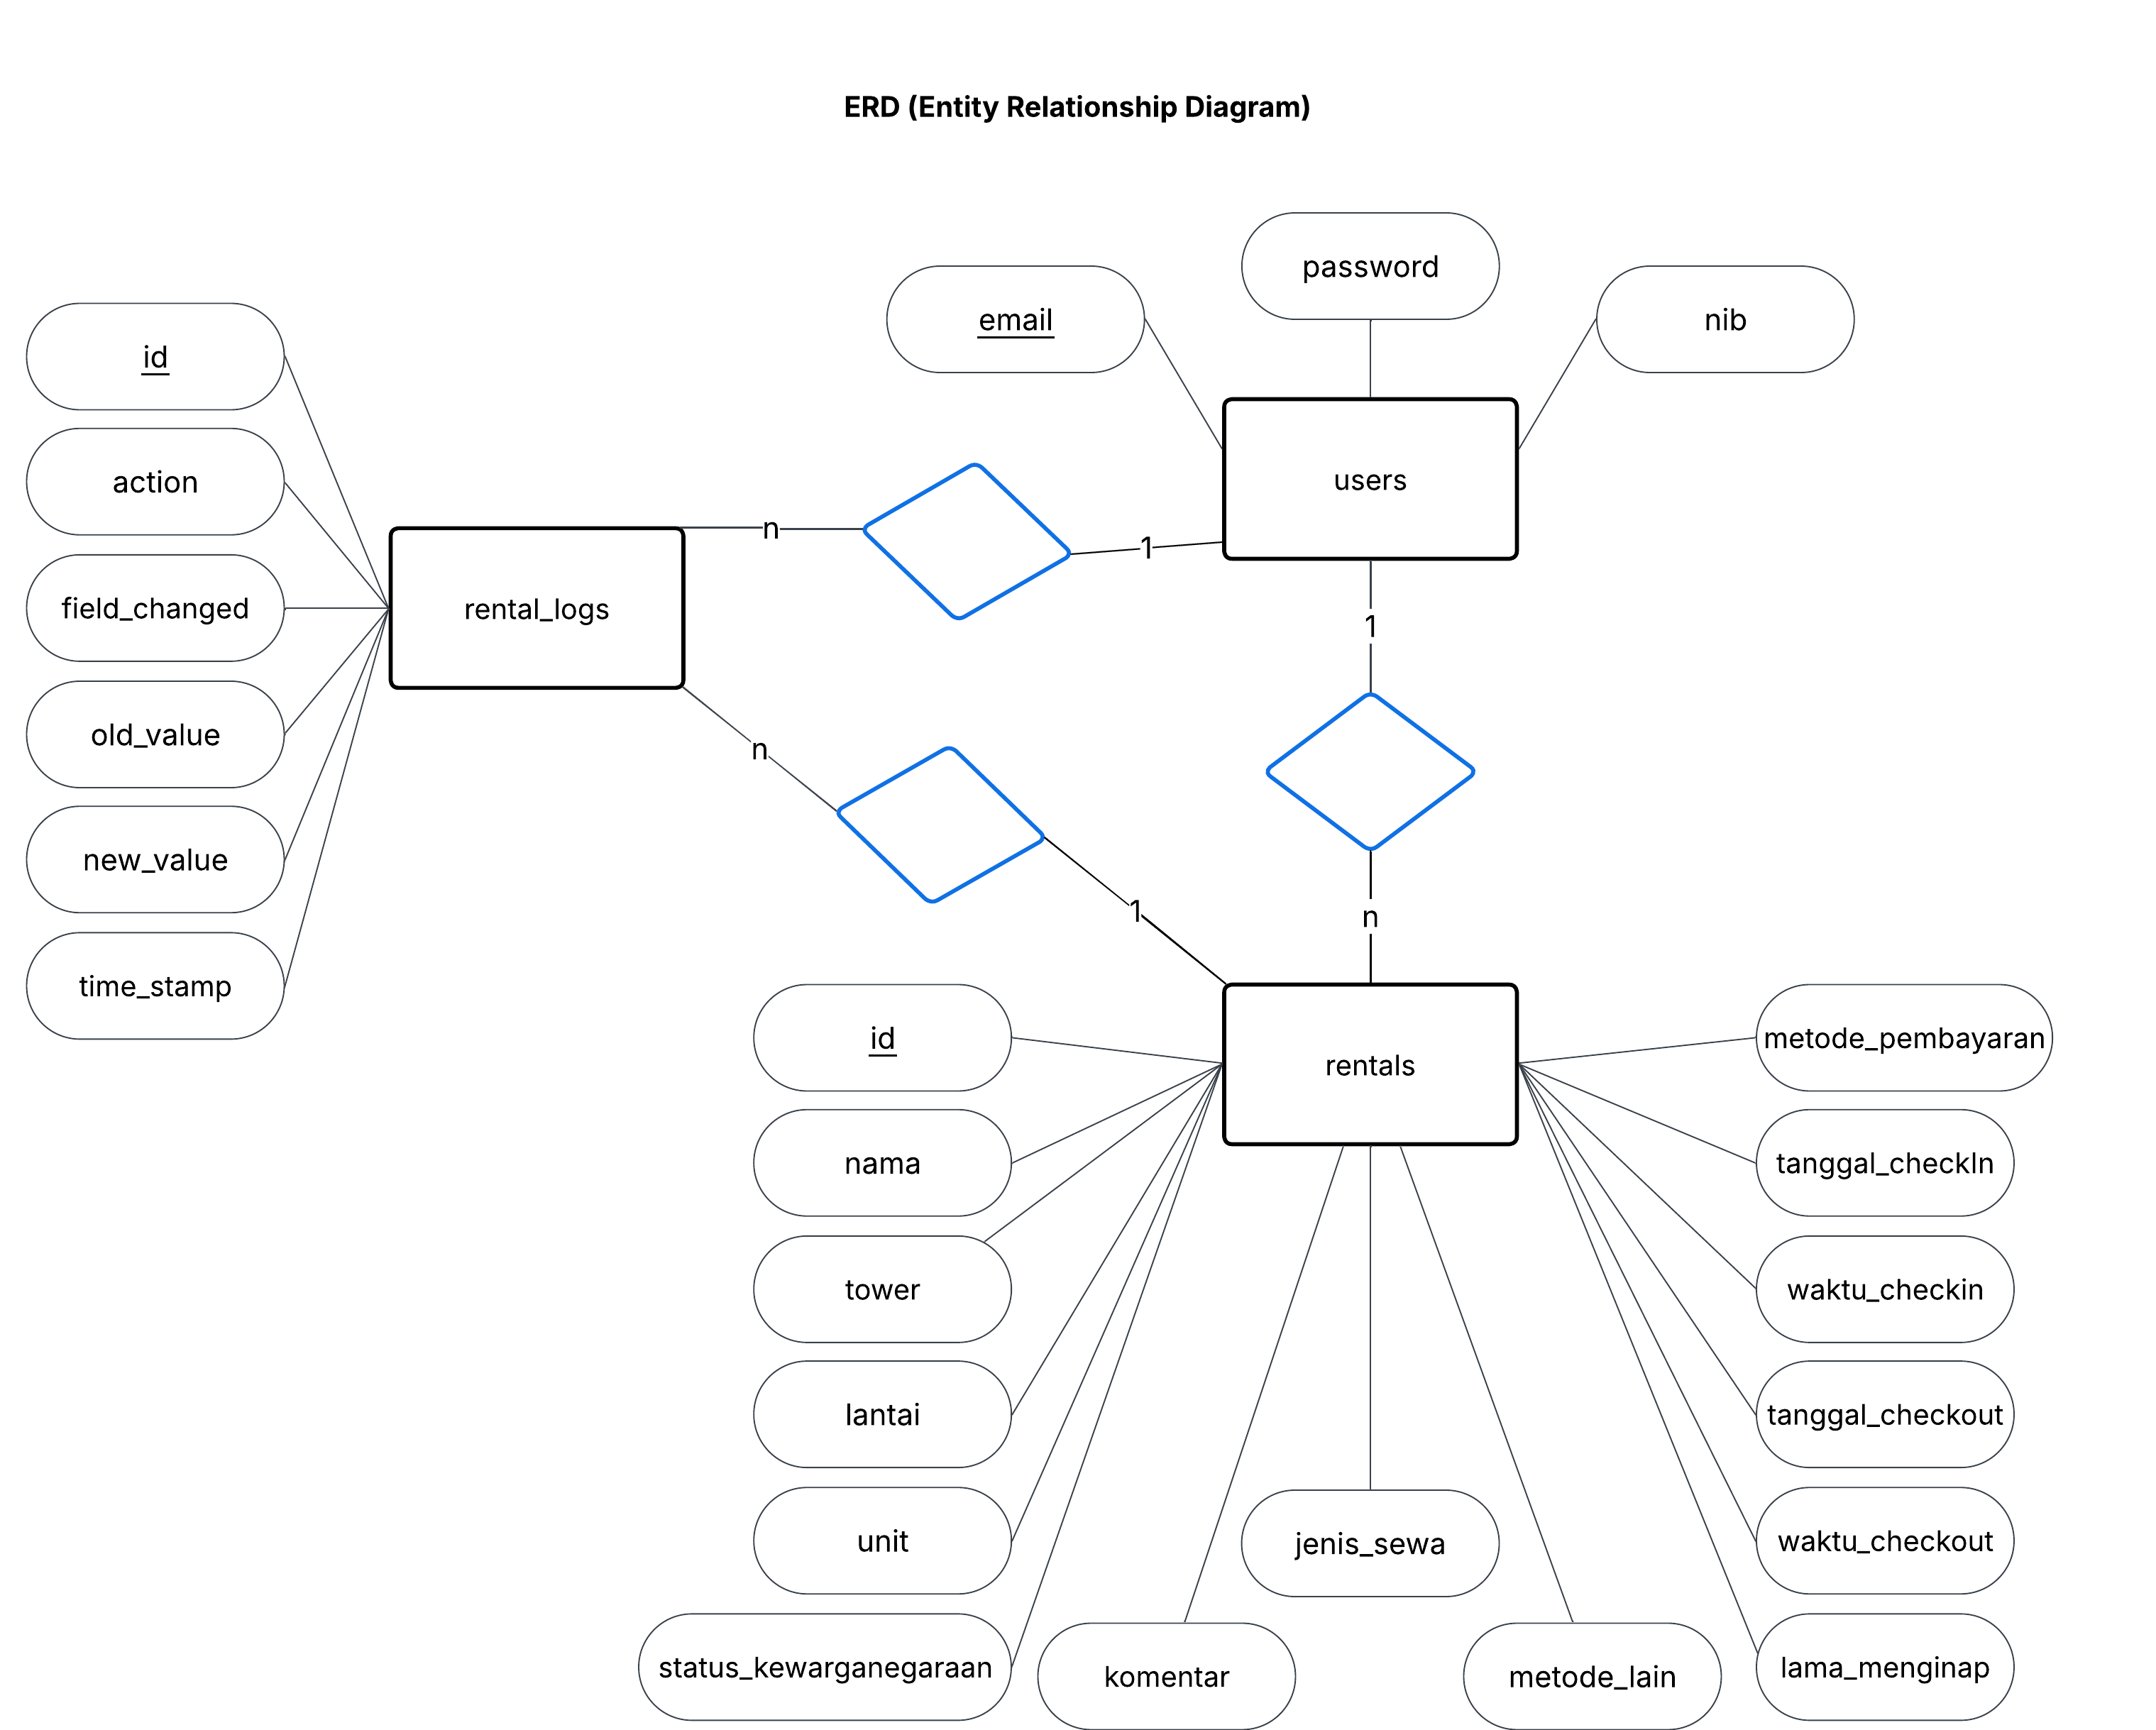
\includegraphics[width=0.8\textwidth]{Gambar/ERD.png}
%     \caption{Entity Relationship Diagram (ERD) Sistem}
%     \label{fig:erd}
% \end{figure}

% Gambar~\ref{fig:erd} menyajikan hubungan antar entitas utama dalam basis data, yaitu tabel \texttt{users}, \texttt{rentals}, dan \texttt{rental\_logs}. Tabel \texttt{users} merepresentasikan Pelaku Komersil yang terdaftar, \texttt{rentals} menyimpan data penyewa, sedangkan \texttt{rental\_logs} mencatat setiap perubahan data yang dilakukan.

% \begin{figure}[H]
%     \centering
%     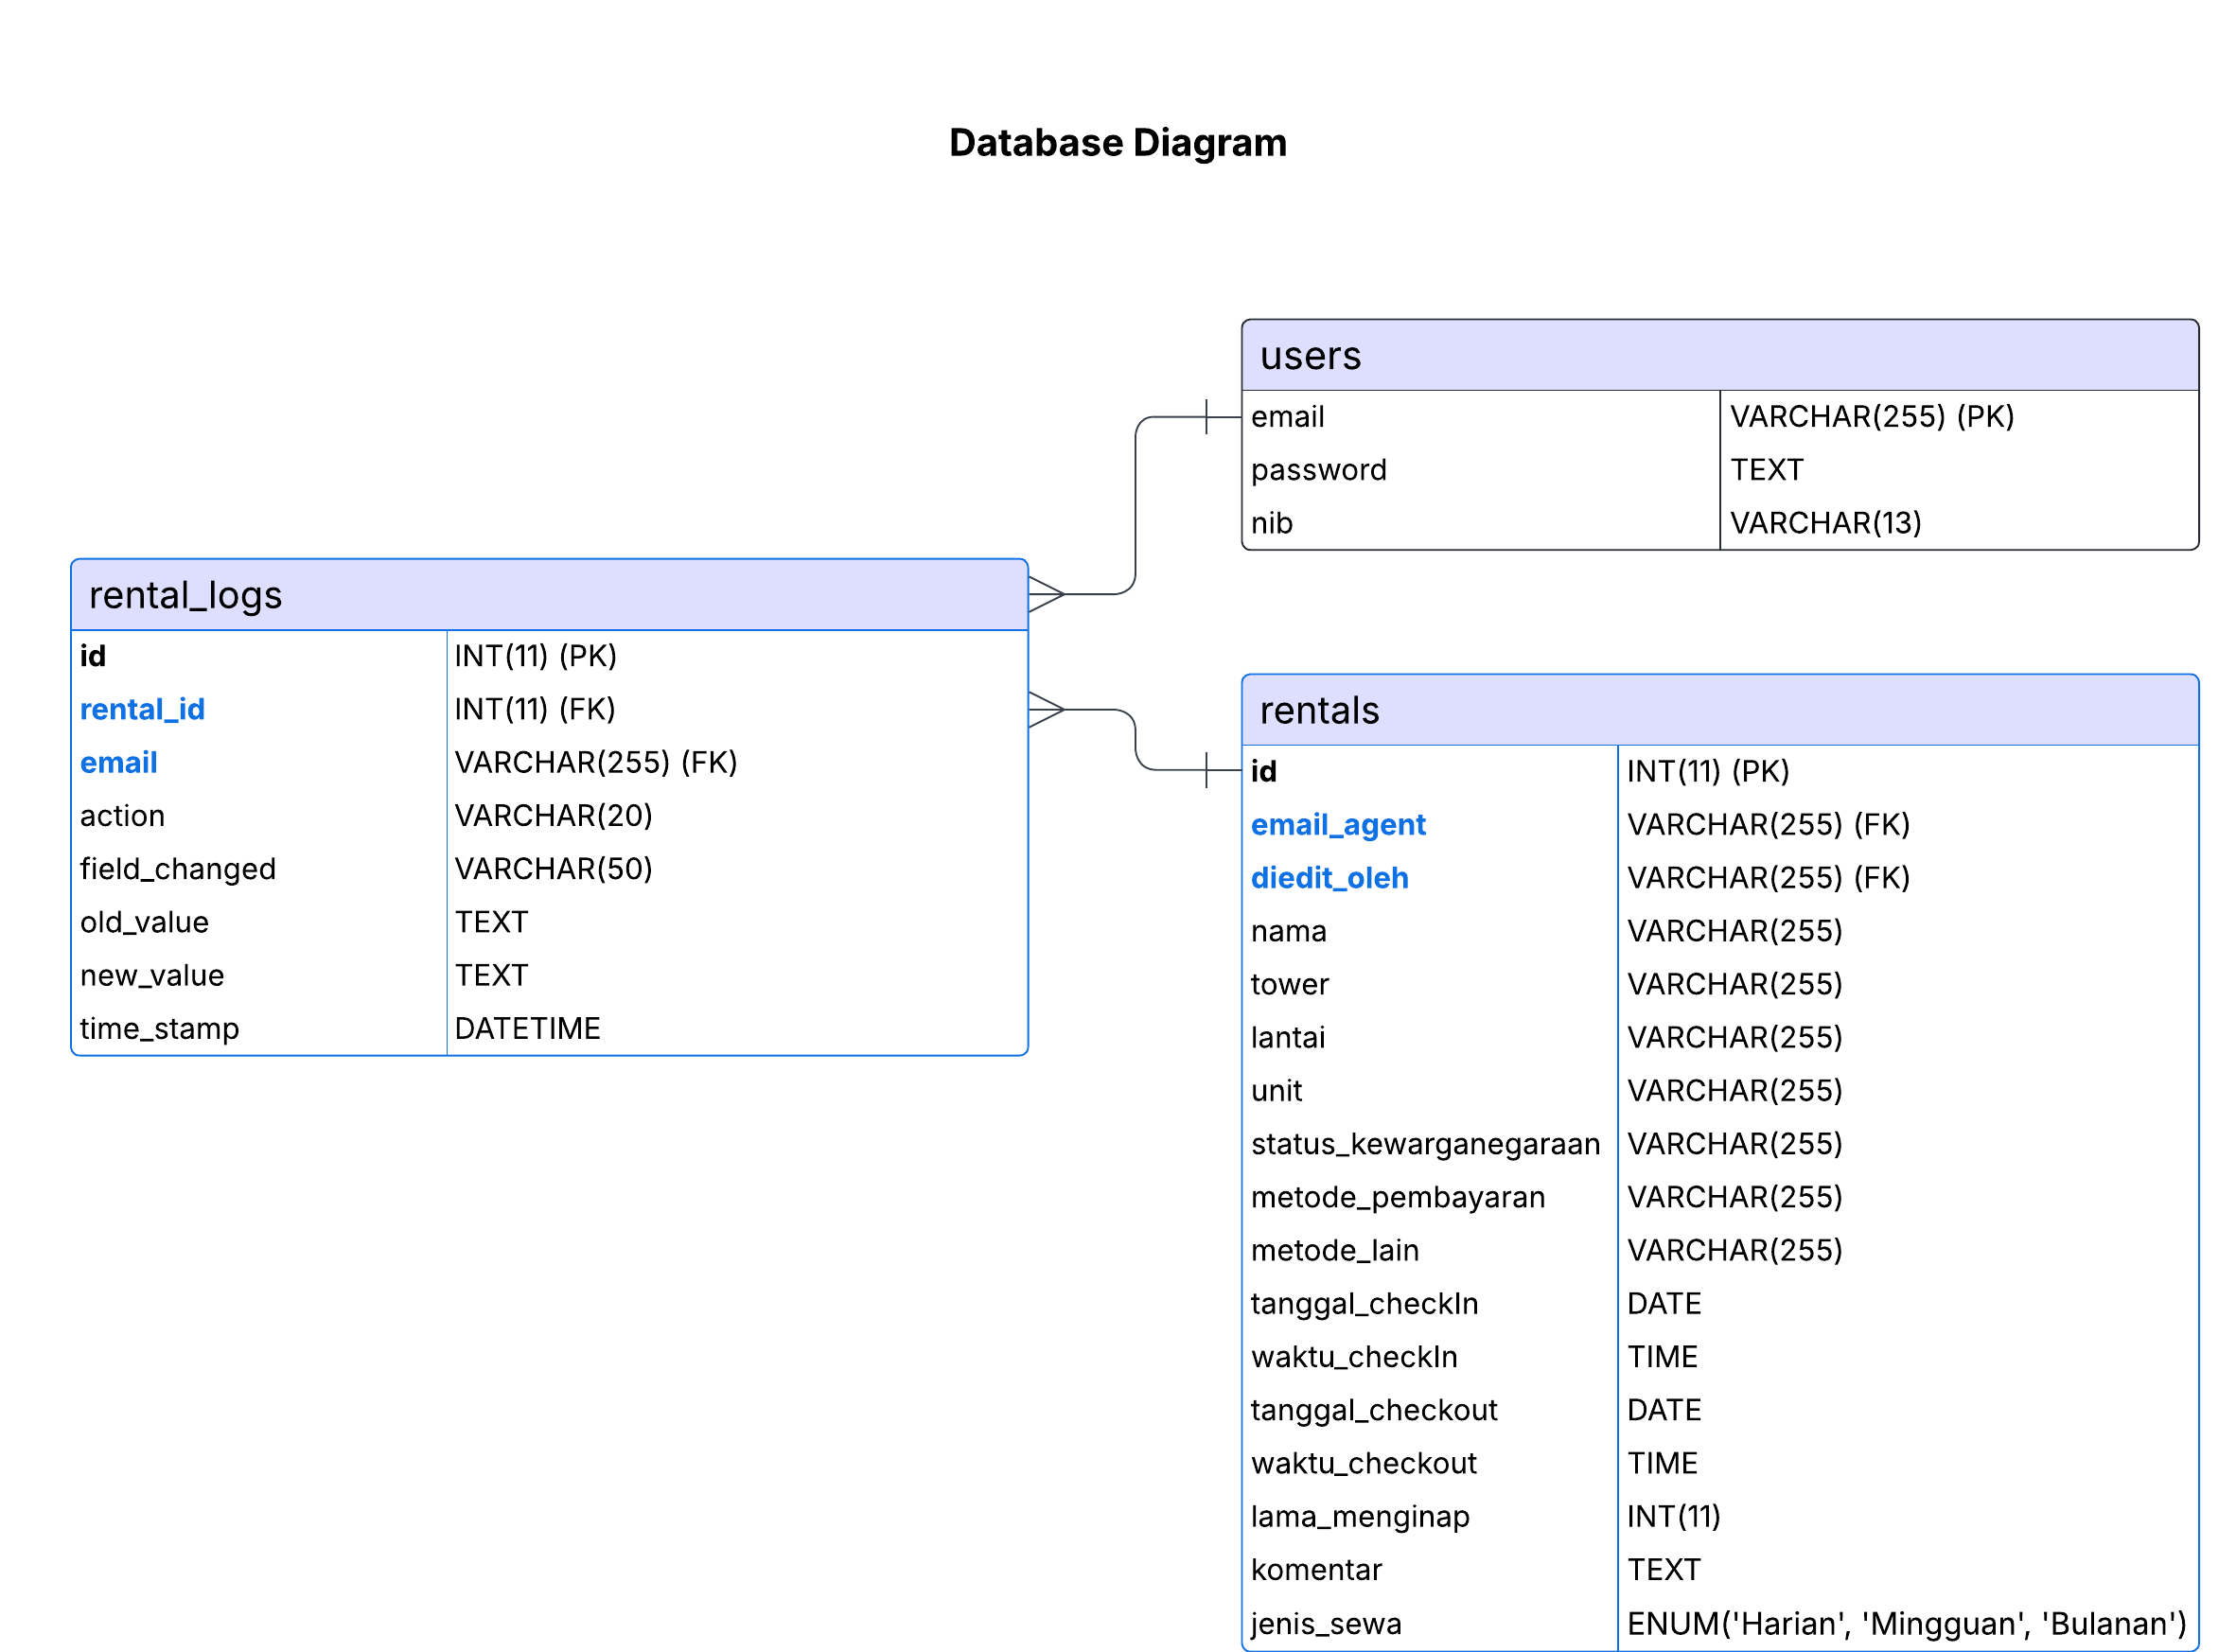
\includegraphics[width=0.7\textwidth, height=0.6\textheight, keepaspectratio]{Gambar/Database Diagram.png}
%     \caption{Database Diagram Sistem}
%     \label{fig:db_diagram}
% \end{figure}

% Gambar~\ref{fig:db_diagram} memperlihatkan struktur tabel dan relasi antar tabel secara fisik di dalam sistem basis data \texttt{MySQL} yang digunakan. Tabel-tabel telah didesain dengan mempertimbangkan kebutuhan pencatatan data yang lengkap, fleksibel, serta mendukung analisis \textit{log} aktivitas dan ekspor data untuk kebutuhan audit atau pelaporan.


% ===========================================================================================


% \subsection{Pemodelan Sistem}
% Pengembangan sistem \textit{data capture} dan deteksi perilaku penyewa ini dilakukan melalui dua tahapan utama, yakni fase sebelum integrasi (berjalan sebagai modul mandiri) dan fase setelah integrasi dengan ekosistem aplikasi {Member} The Jarrdin (\url{https://member.thejarrdin.com/}). Pemodelan alur kerja, interaksi pengguna, serta struktur basis data divisualisasikan melalui {Flowchart}, {Use Case Diagram}, {Entity Relationship Diagram} (ERD), dan Diagram Basis Data.

% \subsubsection{Arsitektur dan Alur Kerja Sistem}
% Pada fase \textbf{sebelum integrasi}, sistem diunggah ke peladen (\textit{server}) SRusun dan beroperasi secara independen. Sistem ini dapat diakses melalui tautan \texttt{steffi.srusun.id}. Pada tahap ini, alur fungsionalitas sistem mencakup pendaftaran akun Pelaku Komersil secara mandiri, proses \textit{login}, pemantauan \textit{dashboard}, pengisian (\textit{input}) data penyewa, hingga peninjauan data penyewaan unit.

% Fase \textbf{setelah integrasi} membawa perubahan signifikan pada arsitektur otorisasi. Pengguna yang mengakses tautan \url{https://visitor.thejarrdin.com/} akan secara otomatis dialihkan ke halaman \textit{login} aplikasi \textit{Member} The Jarrdin. Proses pendaftaran dan \textit{login} mandiri ditiadakan, digantikan oleh mekanisme \textit{Single Sign-On} (SSO) menggunakan token JWT (JSON \textit{Web Token}) dari basis data utama SRusun. Setelah autentikasi berhasil, pengguna dapat mengakses sistem \textit{data capture} ini melalui menu ``Penyewaan Unit''. Alur ini menjadikan operasional lebih ringkas karena sistem langsung mengenali identitas dan peran pengguna dari aplikasi induk tanpa memerlukan autentikasi ganda.

% \begin{figure}[H]
%     \centering
%     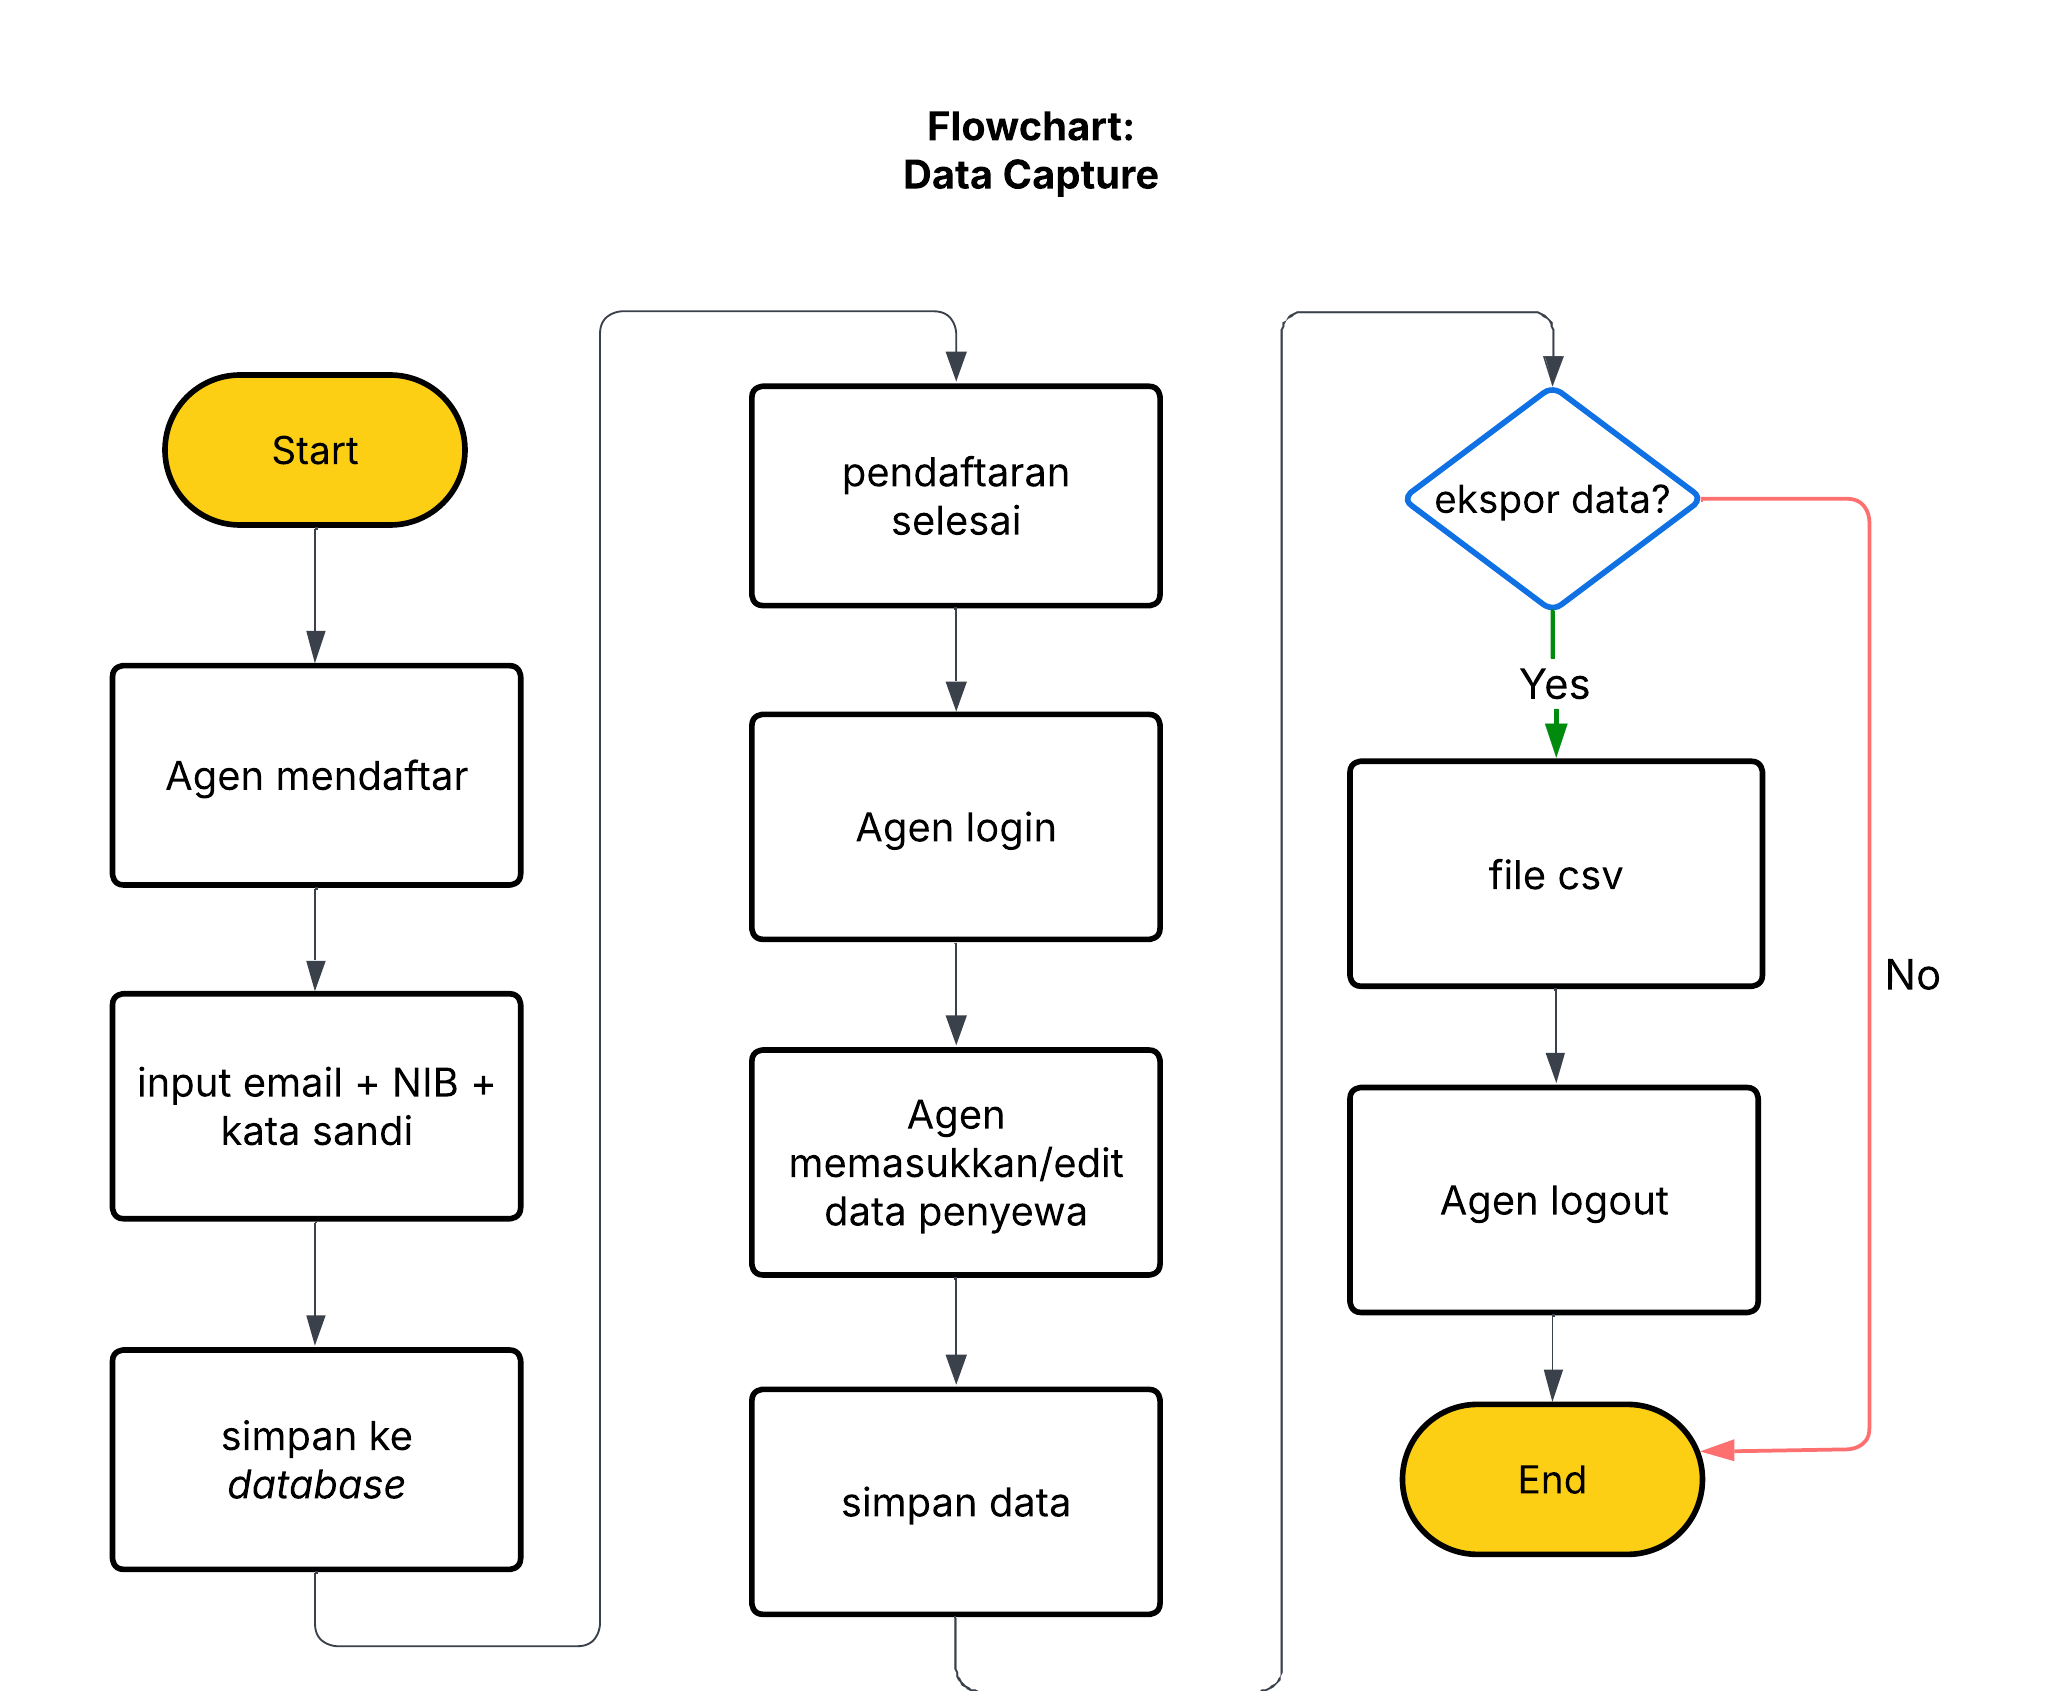
\includegraphics[width=0.7\textwidth]{Gambar/Flowchart Sistem Data Capture.png}
%     \caption{Flowchart untuk Sistem \textit{Data Capture}}
%     \label{fig:flowchart_data_capture}
% \end{figure}

% Gambar~\ref{fig:flowchart_data_capture} menjelaskan alur operasional utama sistem. Bagi pengguna yang telah terautentikasi (baik secara mandiri sebelum integrasi, maupun via token setelah integrasi), sistem memfasilitasi proses input data penyewa, penyimpanan data ke basis data, ekspor data dalam format CSV, serta pencatatan otomatis terhadap seluruh riwayat perubahan data (\textit{audit log}).

% \begin{figure}[H]
%     \centering
%     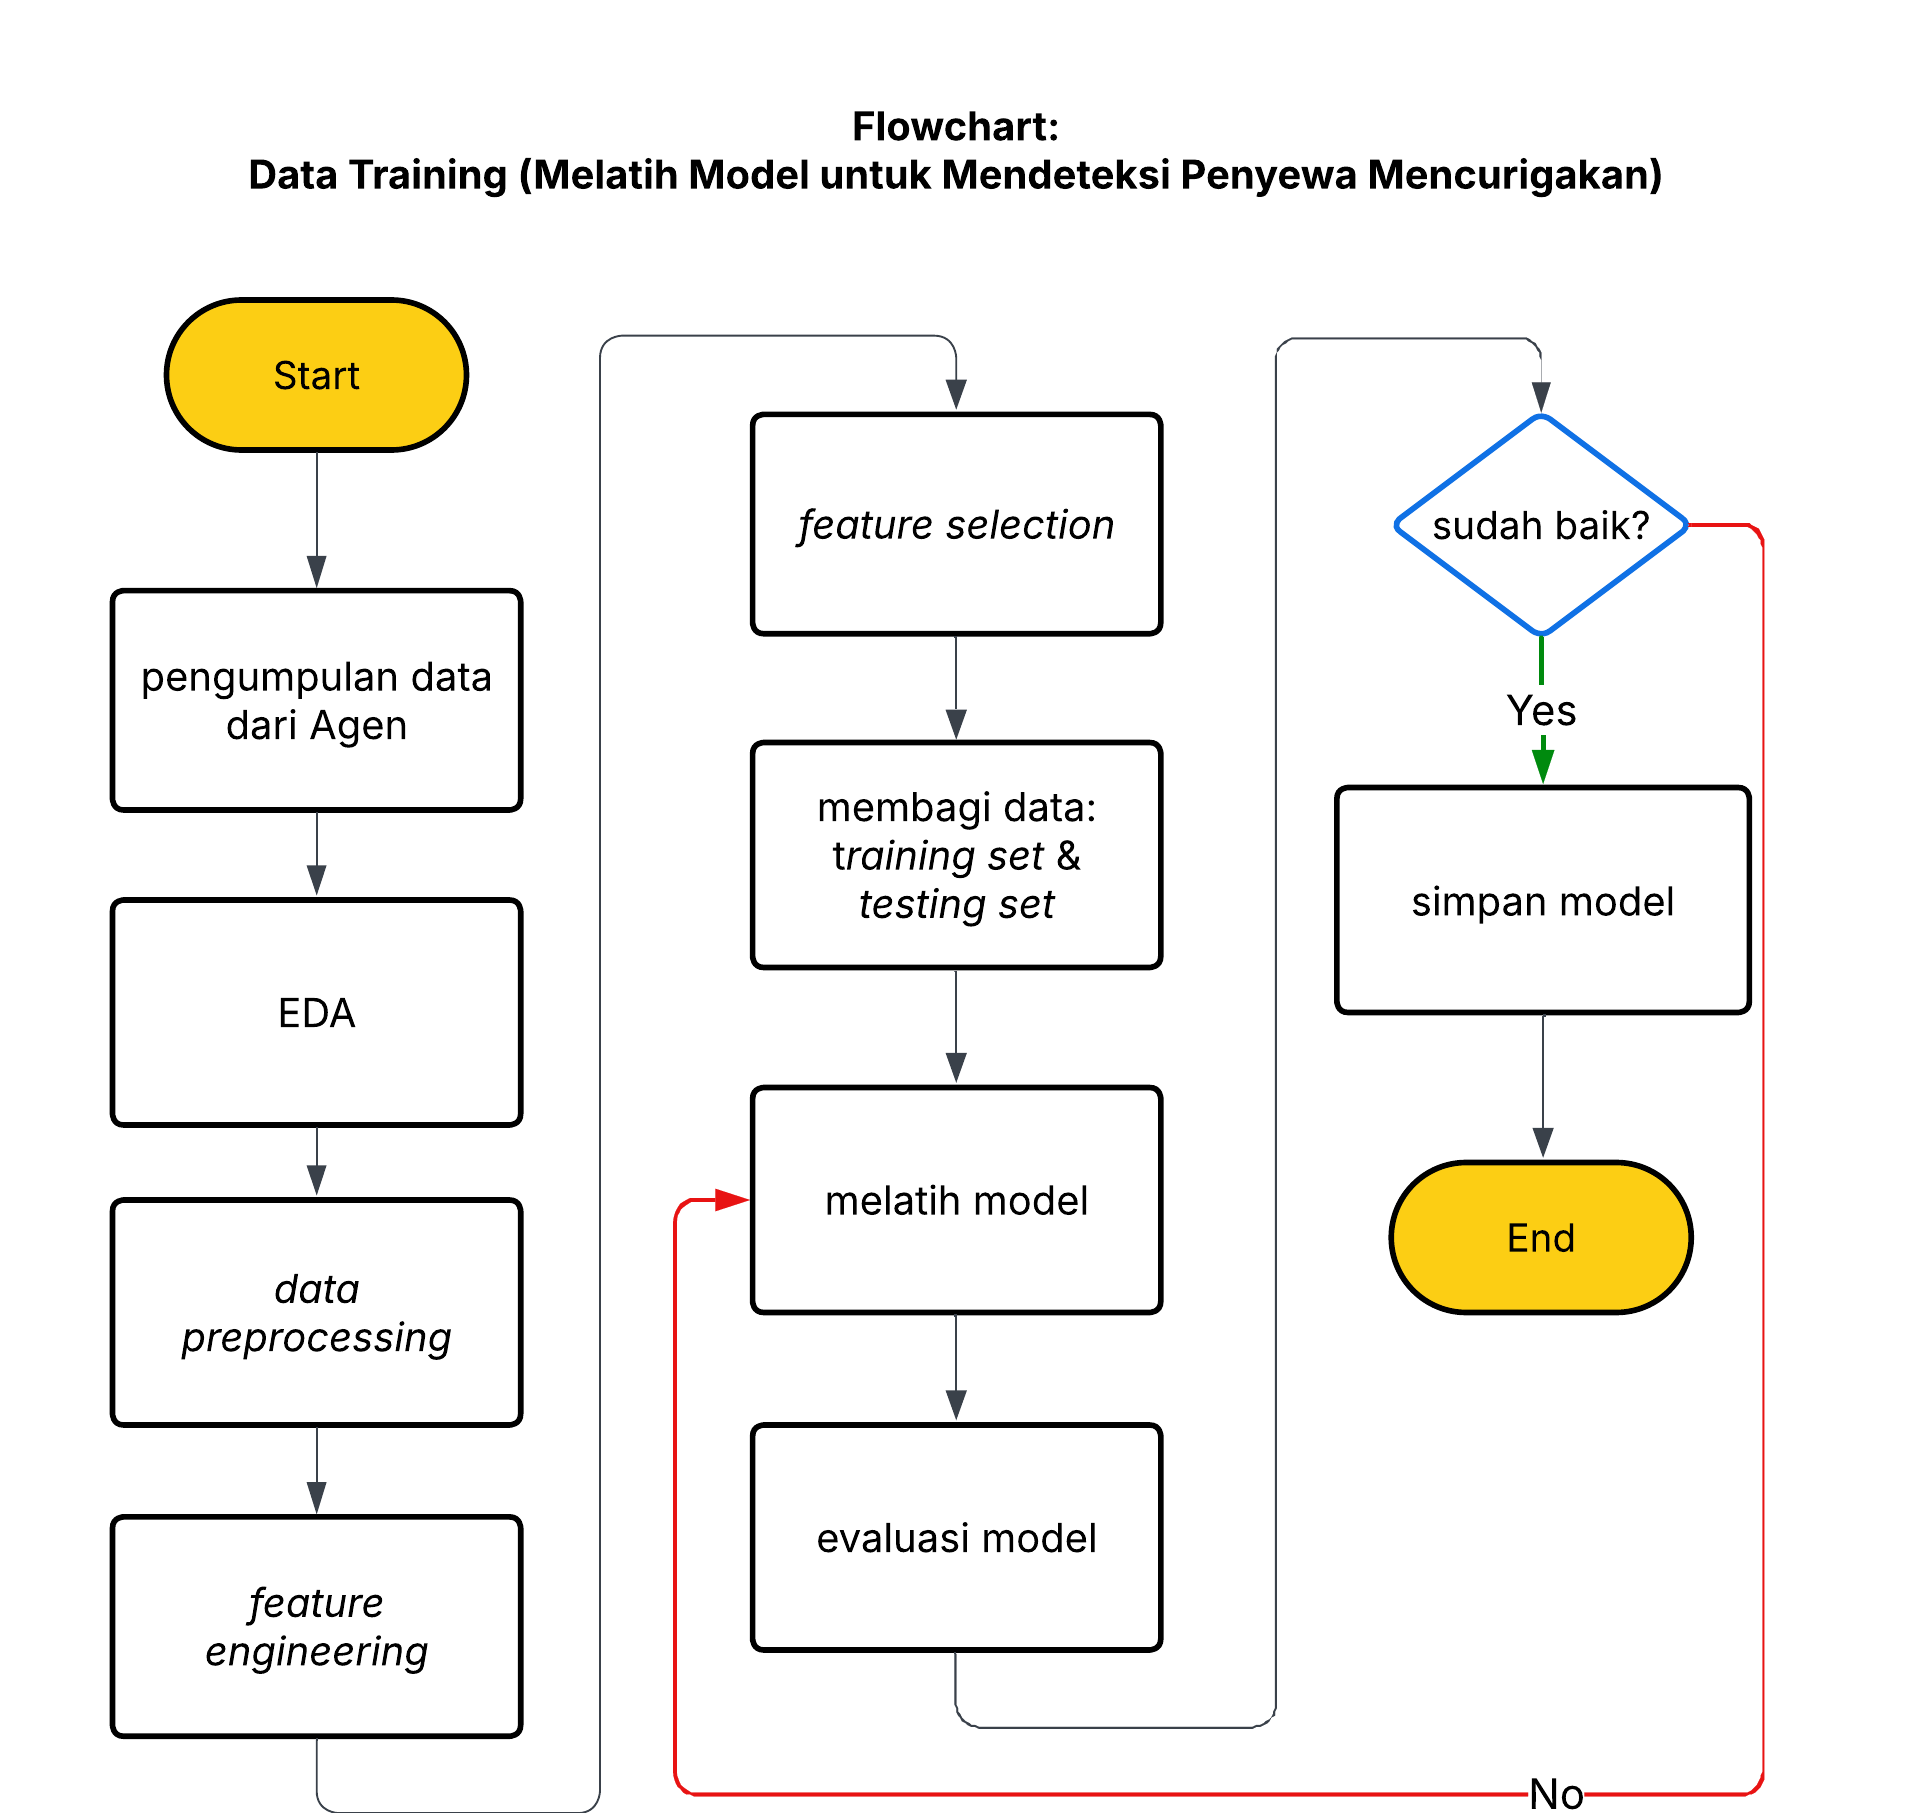
\includegraphics[width=0.7\textwidth]{Gambar/Flowchart Proses Data Training.png}
%     \caption{Flowchart \textit{Data Training}}
%     \label{fig:flowchart_data_training}
% \end{figure}

% Gambar~\ref{fig:flowchart_data_training} menunjukkan proses persiapan data historis penyewa yang telah berhasil dikumpulkan oleh sistem. Data tersebut melalui tahap pra-pemrosesan untuk digunakan sebagai data pelatihan (\textit{training data}) bagi model klasifikasi \textit{machine learning}. Data pelatihan ini menjadi fondasi utama dalam mengenali pola perilaku normal dan anomali penyewa.

% \begin{figure}[H]
%     \centering
%     
\includegraphics[width=0.7\textwidth]{Gambar/Flowchart Proses Analisis & Notif.png}
%     \caption{Flowchart untuk Deteksi Penyewa Mencurigakan}
%     \label{fig:flowchart_deteksi_penyewa_mencurigakan}
% \end{figure}

% Gambar~\ref{fig:flowchart_deteksi_penyewa_mencurigakan} menggambarkan mekanisme inferensi model. Data penyewa baru yang diinputkan akan dianalisis dan diverifikasi oleh algoritma. Jika sistem mendeteksi keberadaan pola atau parameter yang mencurigakan (misalnya metode pembayaran yang tidak biasa, waktu \textit{check-in} di luar jam operasional normal, atau durasi inap yang sangat singkat), maka sistem akan secara otomatis memberikan notifikasi peringatan dini kepada pihak pengelola.

% \subsubsection{Interaksi Pengguna (\textit{Use Case Diagram})}

% \begin{figure}[H]
%     \centering
%     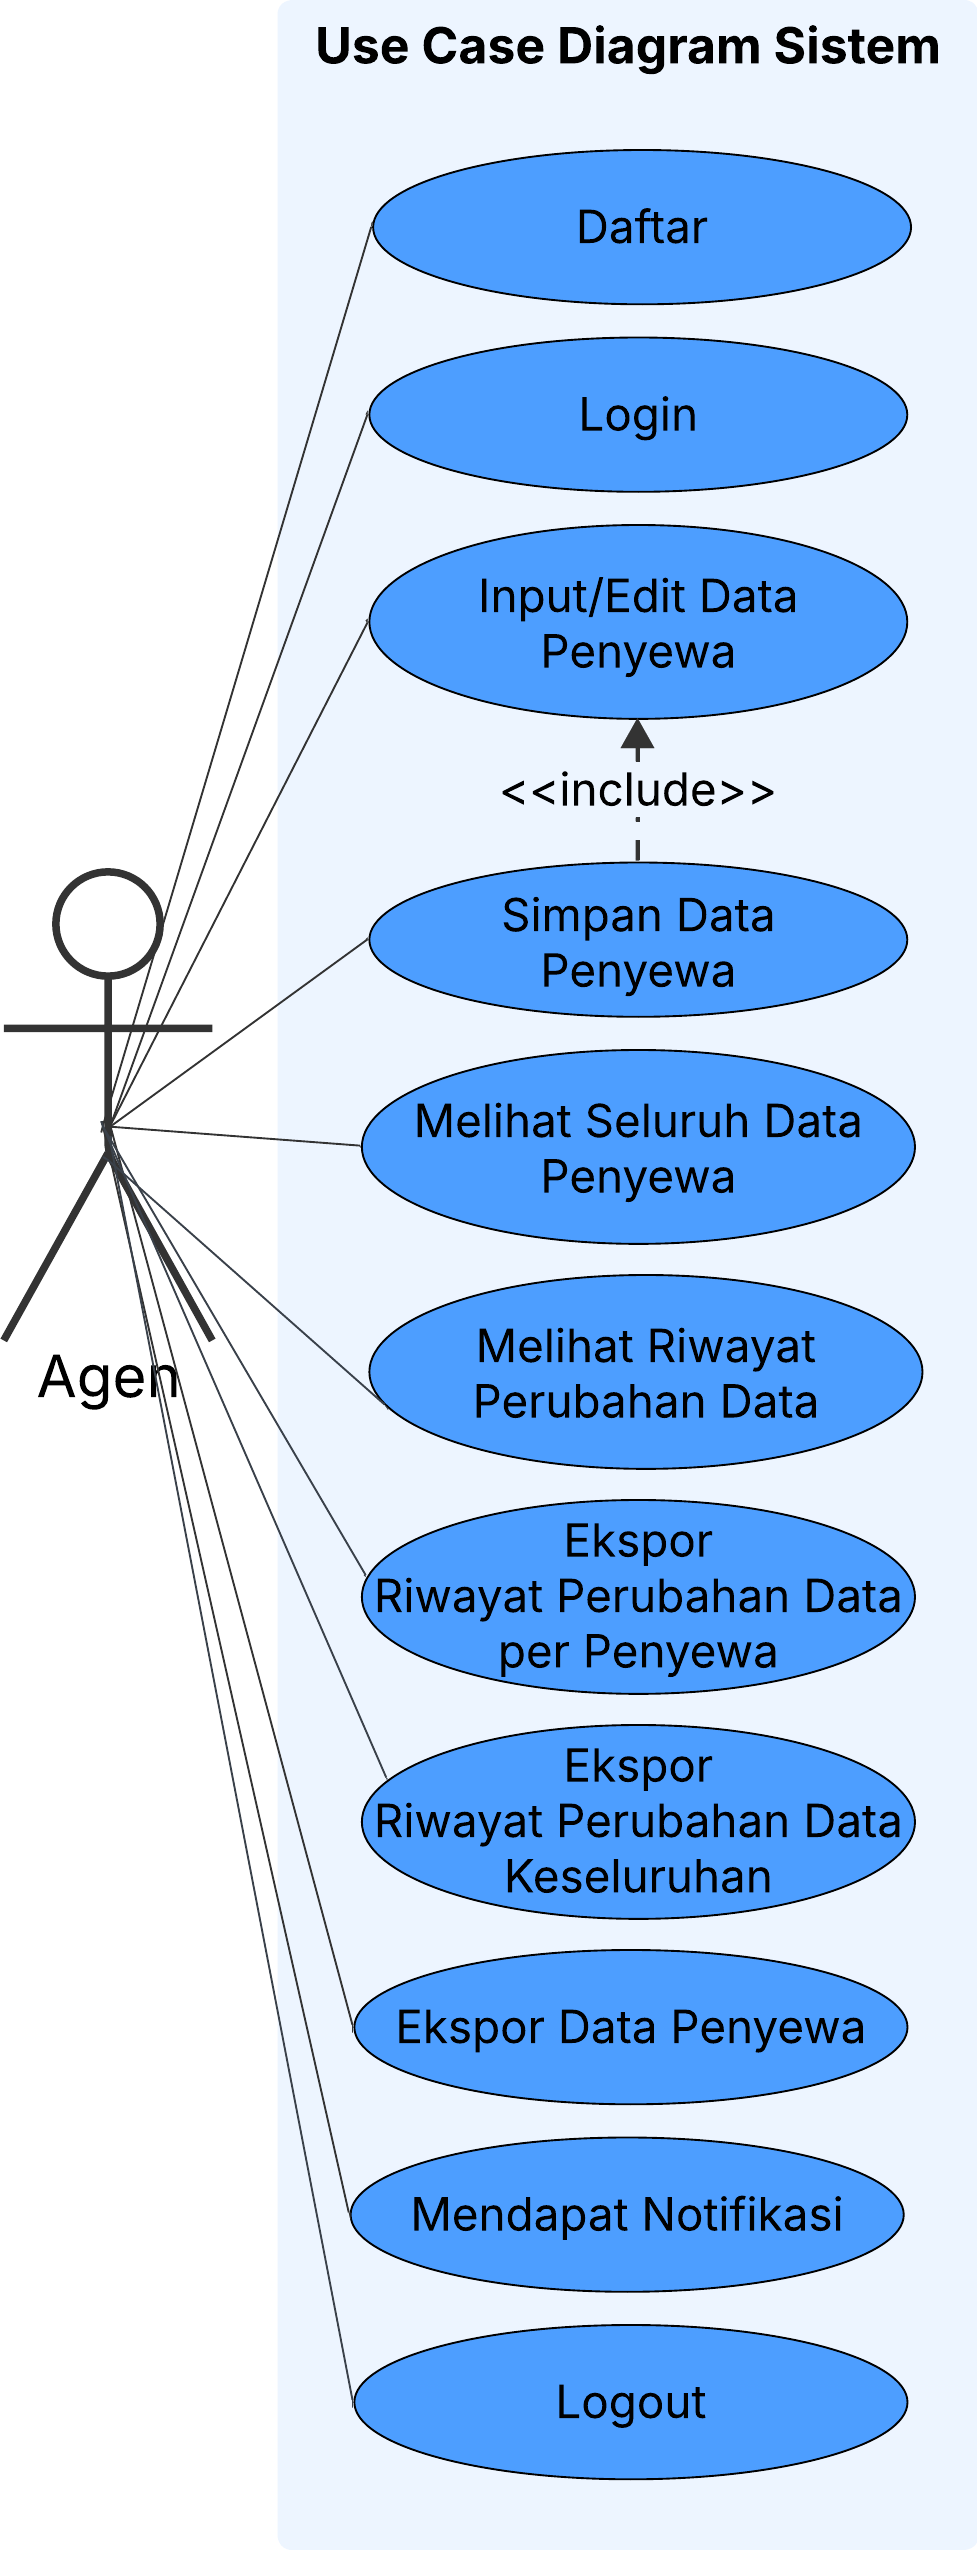
\includegraphics[width=0.47\textwidth, height=0.6\textheight, keepaspectratio]{Gambar/Use Case Diagram System.png}
%     \caption{\textit{Use Case Diagram} Sistem}
%     \label{fig:use_case_data_capture}
% \end{figure}

% Gambar~\ref{fig:use_case_data_capture} mendeskripsikan pemetaan fungsionalitas sistem berdasarkan peran (\textit{role}) aktor. 
% \begin{itemize}
%     \item \textbf{Sebelum Integrasi:} Aktor (Pelaku Komersil dan Pengelola) merupakan entitas lokal yang mendaftar dan dikelola secara mandiri di dalam basis data aplikasi \textit{data capture}.
%     \item \textbf{Setelah Integrasi:} Aktor dan hak aksesnya diwariskan secara langsung dari sistem \textit{Member} The Jarrdin. Pelaku Komersil hanya dapat mengakses dan mengelola data unit miliknya sendiri, sementara Pengelola (Ketua Agen, P3SRS, atau PKJ) diberikan kewenangan administratif untuk melihat rekapitulasi data dari seluruh agen, mengelola master unit, dan meninjau laporan pelanggaran.
% \end{itemize}

% \subsubsection{Struktur Basis Data (ERD dan \textit{Database Diagram})}

% \begin{figure}[H]
%     \centering
%     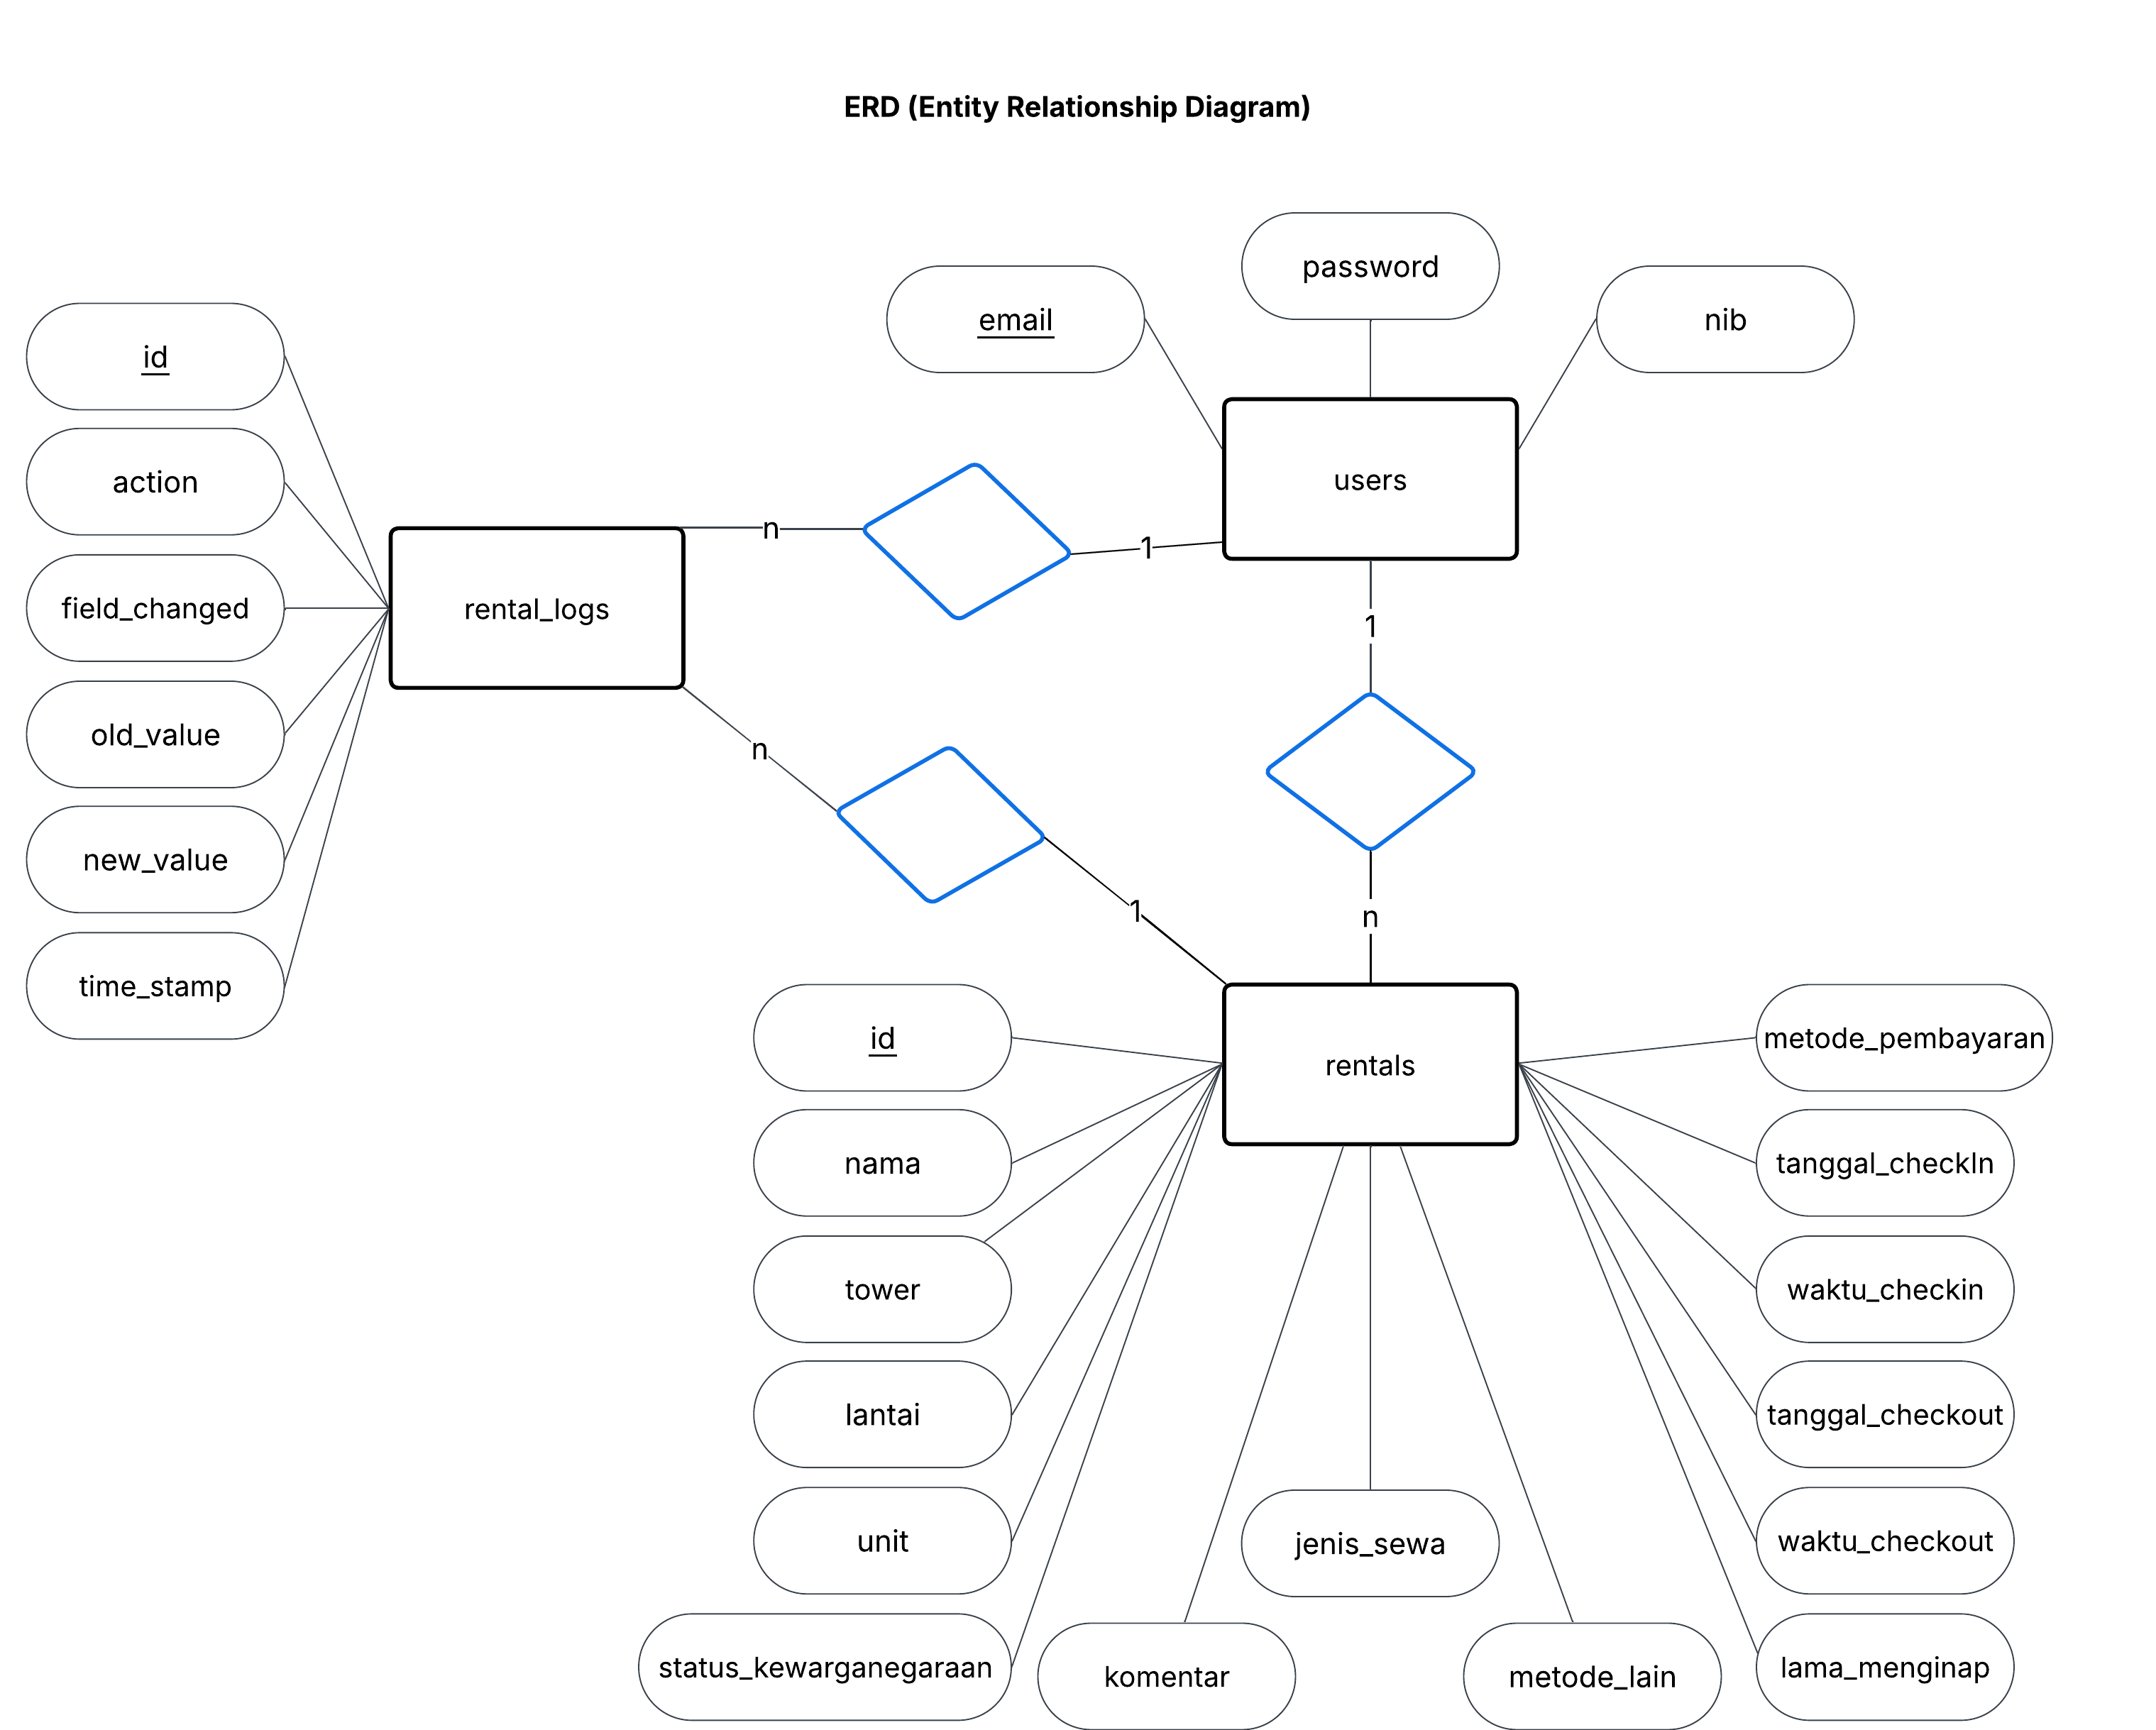
\includegraphics[width=0.8\textwidth]{Gambar/ERD.png}
%     \caption{Entity Relationship Diagram (ERD) Sistem}
%     \label{fig:erd}
% \end{figure}

% Gambar~\ref{fig:erd} menyajikan hubungan konseptual antar-entitas utama dalam sistem. Perubahan struktur basis data juga terjadi seiring dengan proses integrasi:
% \begin{itemize}
%     \item \textbf{Sebelum Integrasi:} Sistem memiliki tabel \texttt{users} tersendiri untuk menyimpan kredensial Pelaku Komersil dan Pengelola yang terelasi langsung dengan tabel \texttt{rentals}.
%     \item \textbf{Setelah Integrasi:} Tabel \texttt{users} lokal digantikan oleh tabel \texttt{pengguna}, \texttt{role}, dan \texttt{pengguna\_role} yang tersentralisasi pada basis data SRusun. Relasi tabel \texttt{rentals} (data penyewa), \texttt{units} (data kamar), \texttt{violations} (data pelanggaran visual), dan \texttt{rental\_logs} (riwayat perubahan) dikaitkan menggunakan kunci tamu (\textit{foreign key}) berupa \texttt{user\_email} yang merujuk pada identitas pengguna di sistem induk.
% \end{itemize}

% \begin{figure}[H]
%     \centering
%     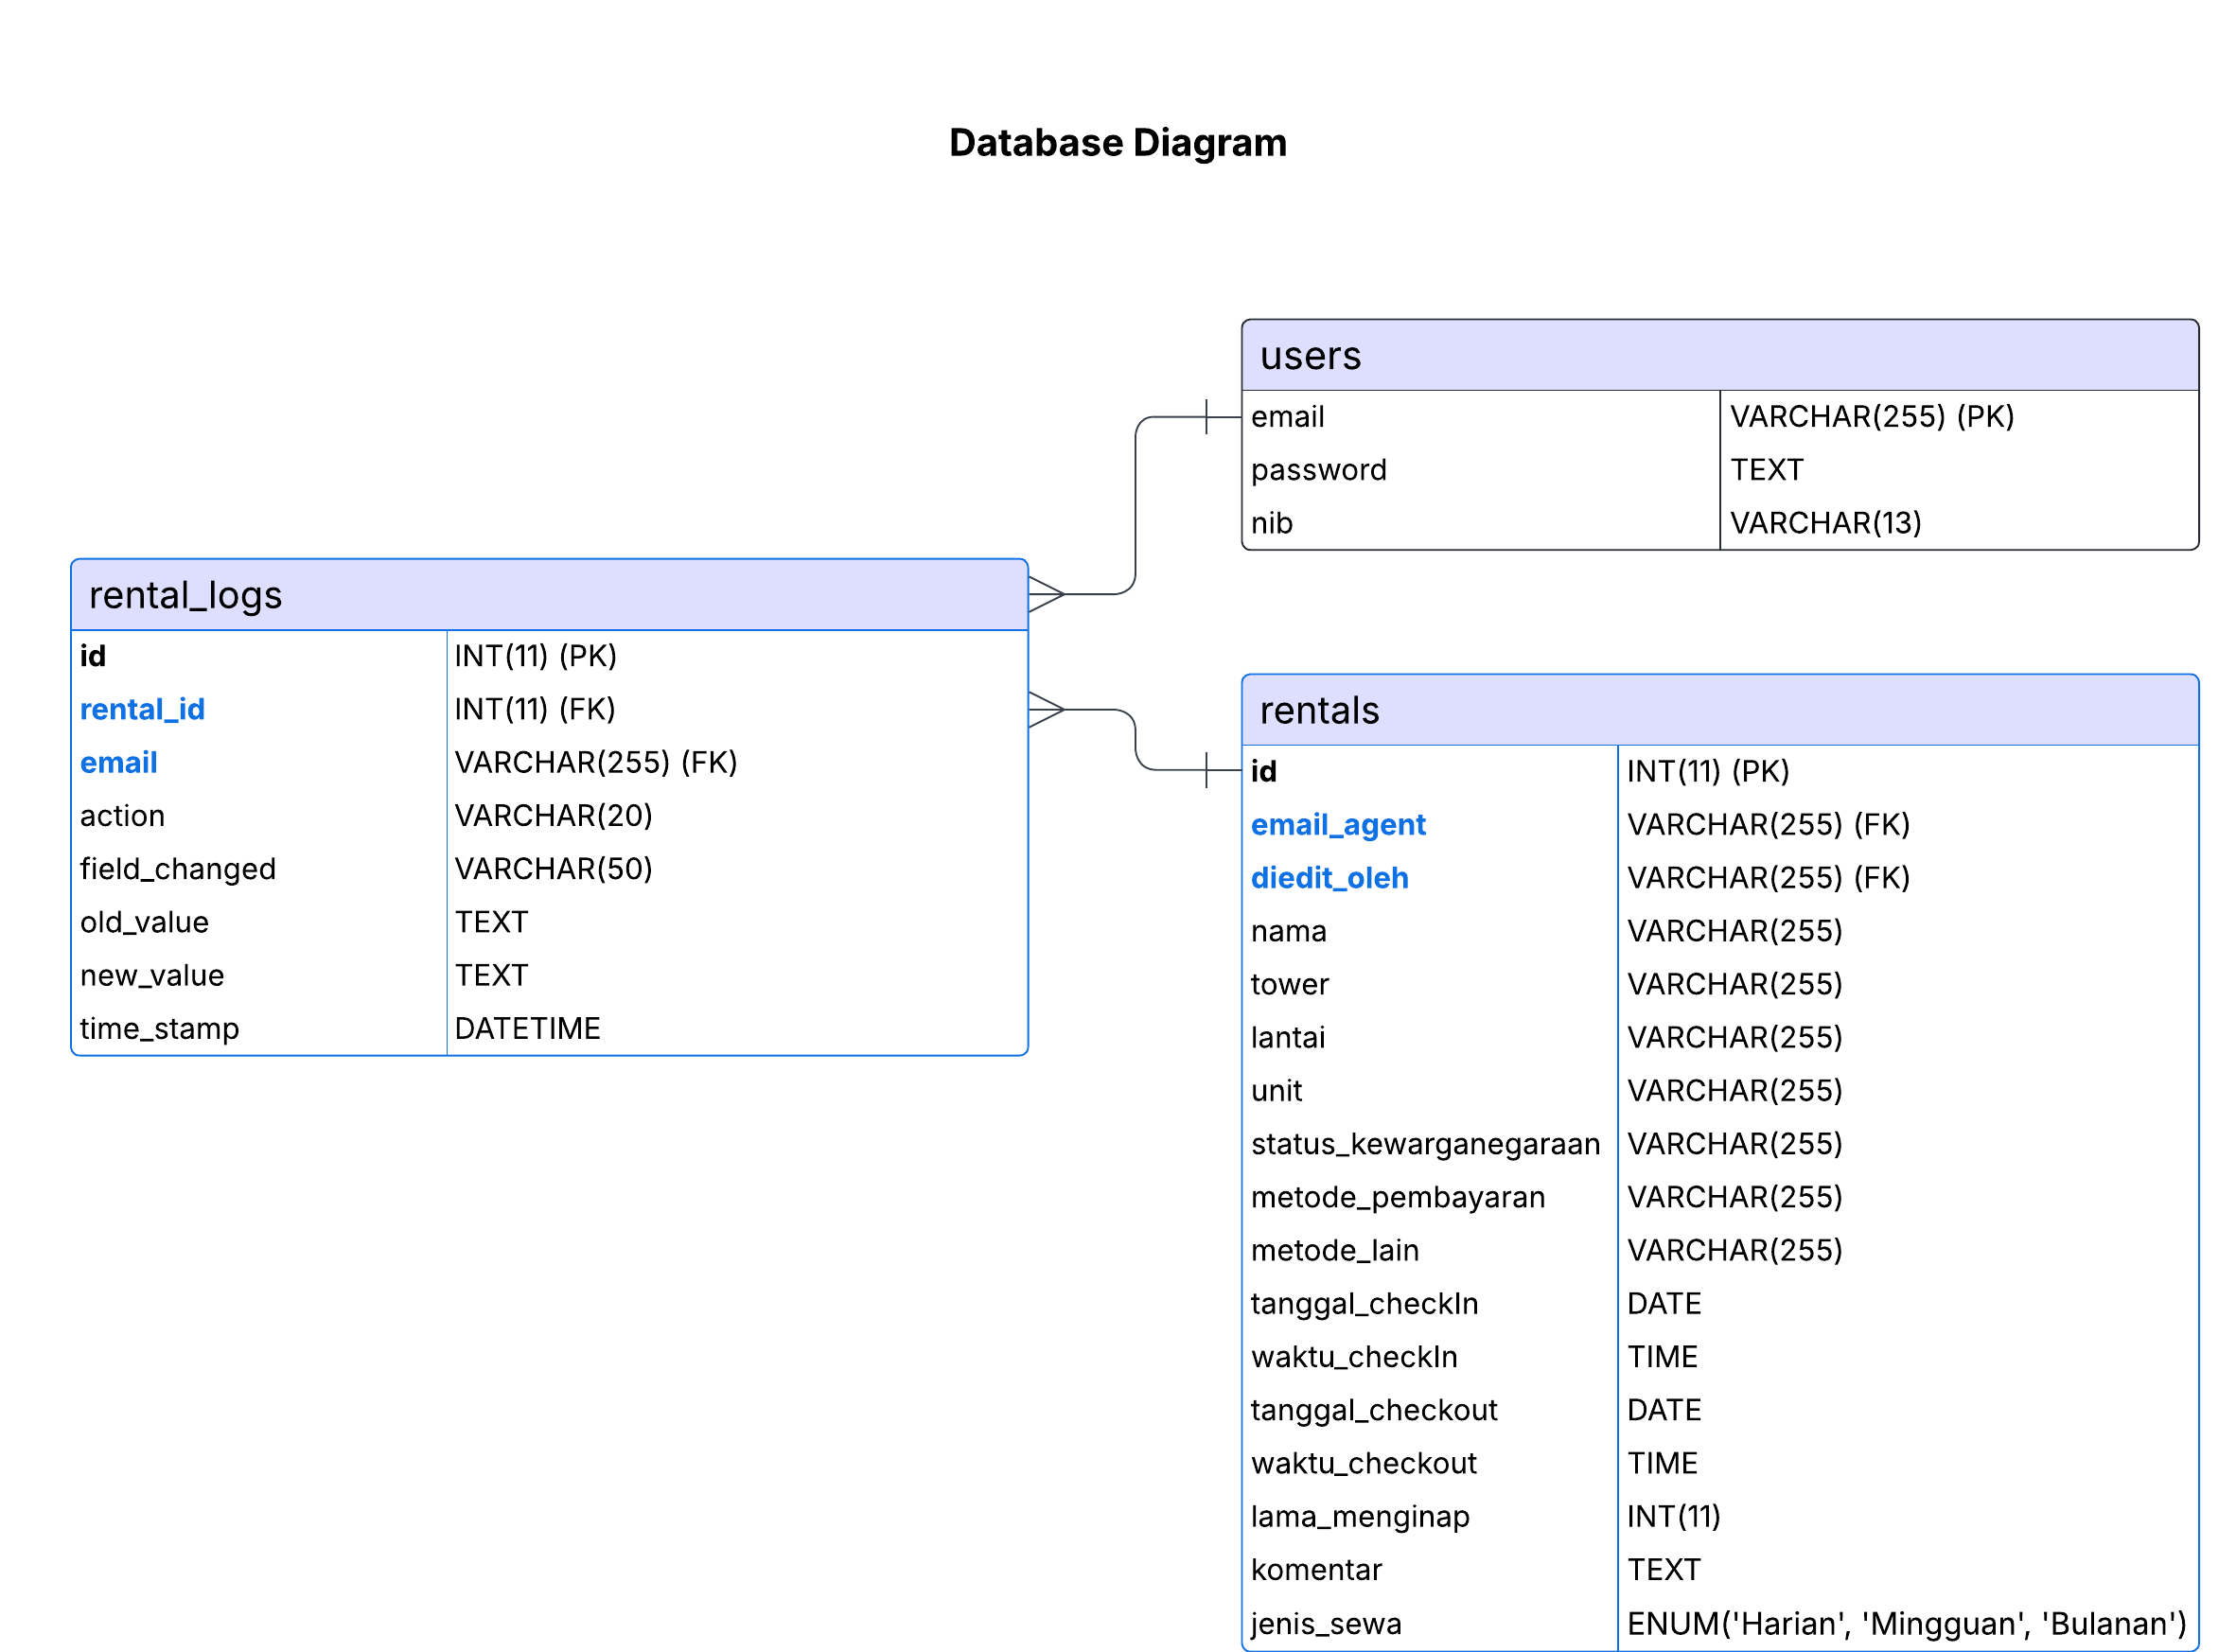
\includegraphics[width=0.7\textwidth, height=0.6\textheight, keepaspectratio]{Gambar/Database Diagram.png}
%     \caption{Database Diagram Sistem Terintegrasi}
%     \label{fig:db_diagram}
% \end{figure}

% Gambar~\ref{fig:db_diagram} memperlihatkan skema fisik (\textit{physical data model}) dari tabel-tabel di dalam sistem basis data MySQL setelah proses integrasi selesai. Desain skema ini telah dioptimalkan untuk memastikan integritas data (melalui relasi antartabel), mendukung penyimpanan data kualitatif (tabel pelanggaran), pencatatan \textit{log} aktivitas yang permanen (audit), serta memfasilitasi ekstraksi data yang efisien untuk keperluan pelatihan model \textit{machine learning}.

% =========================================================================================

\subsection{Pemodelan Sistem}
Pengembangan sistem \textit{data capture} dan deteksi perilaku penyewa ini dilakukan melalui dua tahapan utama, yakni fase sebelum integrasi (berjalan sebagai modul mandiri) dan fase setelah integrasi dengan ekosistem aplikasi \textit{Member} The Jarrdin (\url{https://member.thejarrdin.com/}). Pemodelan alur kerja, interaksi pengguna, serta struktur basis data divisualisasikan melalui {Flowchart}, {Use Case Diagram}, {Entity Relationship Diagram} (ERD), dan Diagram Basis Data.

\subsubsection{Fase Sebelum Integrasi (Modul Mandiri)}
Pada fase ini, sistem diunggah ke {server} SRusun dan beroperasi secara independen. Sistem ini dapat diakses melalui tautan \texttt{steffi.srusun.id}.

\begin{enumerate}
    % \item \textbf{Arsitektur dan Alur Kerja Sistem} \\
    % Alur fungsionalitas sistem pada tahap ini menuntut pengguna untuk melakukan autentikasi secara mandiri. Alur operasional utamanya mencakup pendaftaran akun Pelaku Komersil, proses \textit{login}, pemantauan \textit{dashboard}, pengisian (\textit{input}) data penyewa, hingga peninjauan data penyewaan unit. 

    % \begin{figure}[H]
    %     \centering
    %     \includegraphics[width=0.7\textwidth]{Gambar/Flowchart Sistem Data Capture Sebelum.png}
    %     \caption{Flowchart untuk Sistem \textit{Data Capture} (Sebelum Integrasi)}
    %     \label{fig:flowchart_data_capture_sebelum}
    % \end{figure}
    
    

    \item \textbf{Interaksi Pengguna (\textit{Use Case Diagram})}
    \begin{figure}[H]
        \centering
        \includegraphics[width=0.47\textwidth, height=0.6\textheight, keepaspectratio]{Gambar/Use Case Diagram System Sebelum.png}
        \caption{\textit{Use Case Diagram} Sistem (Sebelum Integrasi)}
        \label{fig:use_case_sebelum}
    \end{figure}
    Gambar~\ref{fig:use_case_sebelum} mendeskripsikan pemetaan fungsionalitas sistem berdasarkan peran (\textit{role}) dari masing-masing aktor. Pada fase ini, aktor (Pelaku Komersil dan Pengelola) merupakan entitas lokal dikelola secara terpisah di dalam basis data aplikasi \textit{data capture}. Alur sistem mewajibkan pengguna untuk memiliki akun sebelum dapat mengakses fungsionalitas aplikasi. Pelaku Komersil yang belum memiliki akun diharuskan melakukan pendaftaran mandiri menggunakan \textit{email}, Nomor Induk Berusaha (NIB), dan kata sandi (\textit{password}). Di sisi lain, akun untuk pihak Pengelola (Ketua Agen, PKJ, dan P3SRS) telah dikonfigurasi dan dibuatkan sebelumnya oleh administrator. Setelah proses \textit{login} berhasil dilakukan, sistem memfasilitasi pengguna untuk melakukan pemantauan \textit{dashboard}, pengisian (\textit{input}) data penyewa, penyimpanan data ke basis data lokal, penarikan (ekspor) data dalam format CSV, serta pencatatan otomatis terhadap seluruh riwayat perubahan data melalui \textit{audit log}.

    \item \textbf{Struktur Basis Data (ERD dan \textit{Database Diagram})}
    \begin{figure}[H]
        \centering
        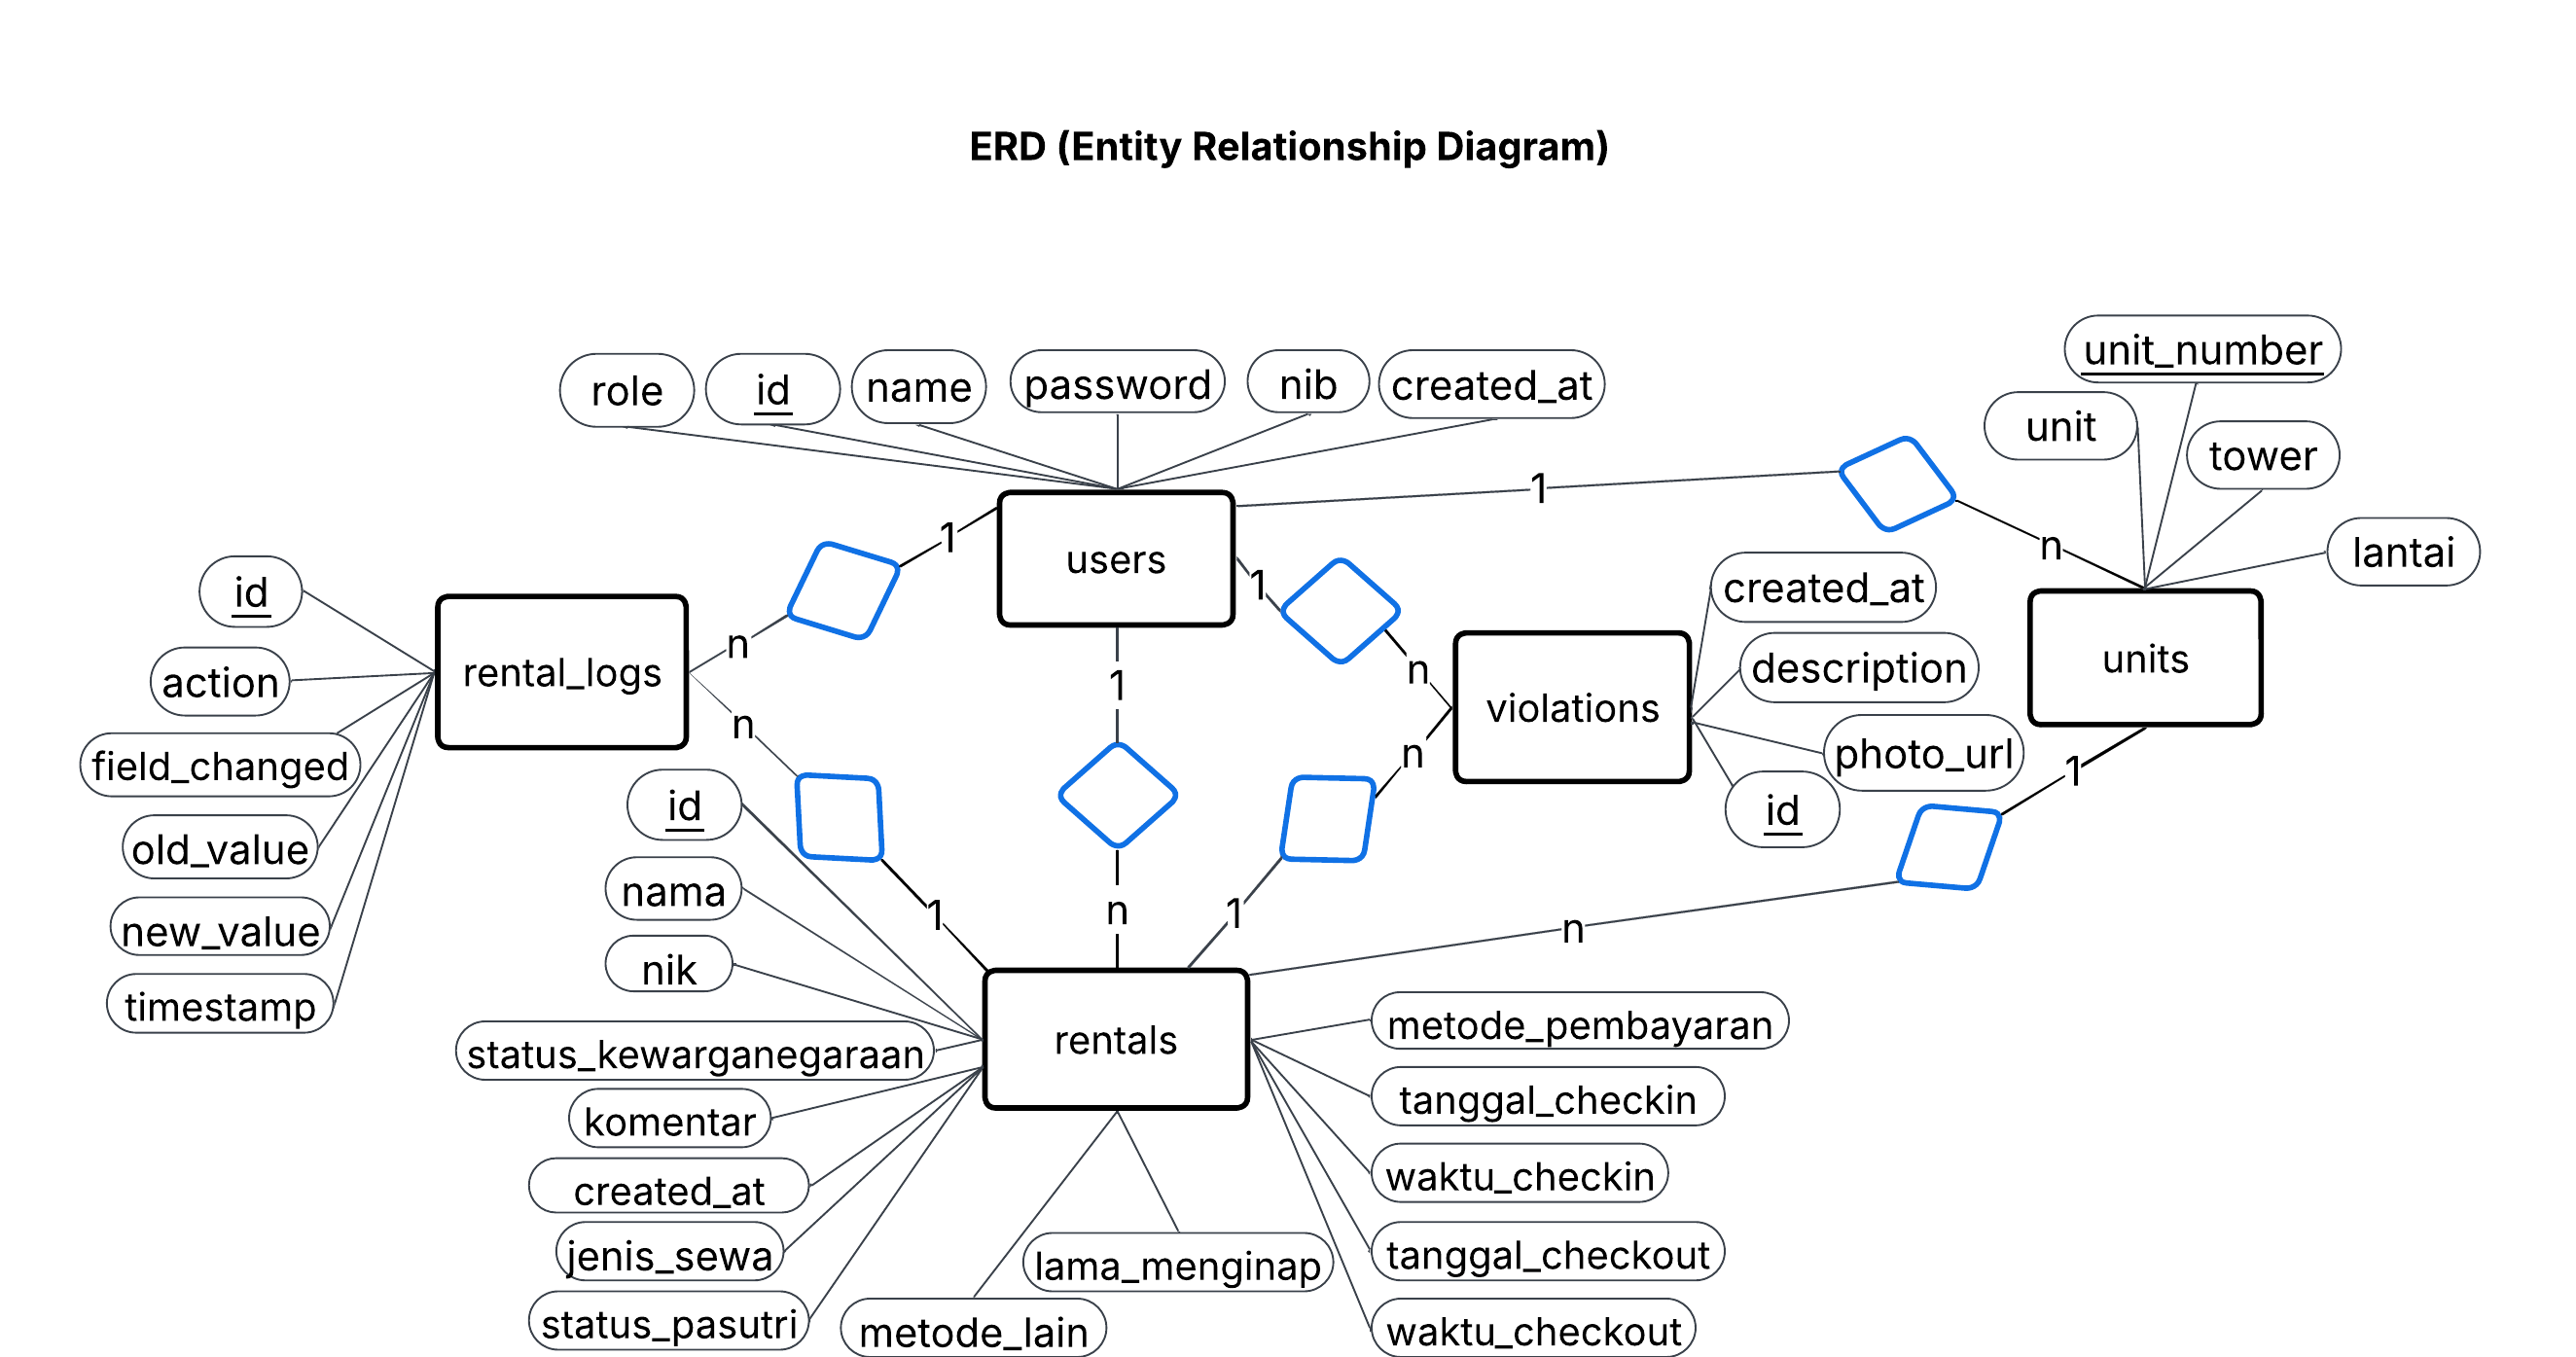
\includegraphics[width=0.8\textwidth]{Gambar/ERD Sebelum.png}
        \caption{Entity Relationship Diagram (ERD) Sistem (Sebelum Integrasi)}
        \label{fig:erd_sebelum}
    \end{figure}
    Seperti yang terlihat pada ERD di Gambar~\ref{fig:erd_sebelum}, arsitektur data bersifat mandiri dan terdiri atas lima tabel utama, yakni \texttt{users}, \texttt{rentals}, \texttt{rental\_logs}, \texttt{units}, serta \texttt{violations}. Sistem memiliki tabel \texttt{users} tersendiri untuk menyimpan kredensial Pelaku Komersil dan Pengelola. Tabel \texttt{users} ini terelasi langsung dengan tabel-tabel operasional, khususnya tabel \texttt{rentals}, untuk mengaitkan data penyewaan beserta riwayat unit dengan entitas penggunanya secara lokal.

    \begin{figure}[H]
        \centering
        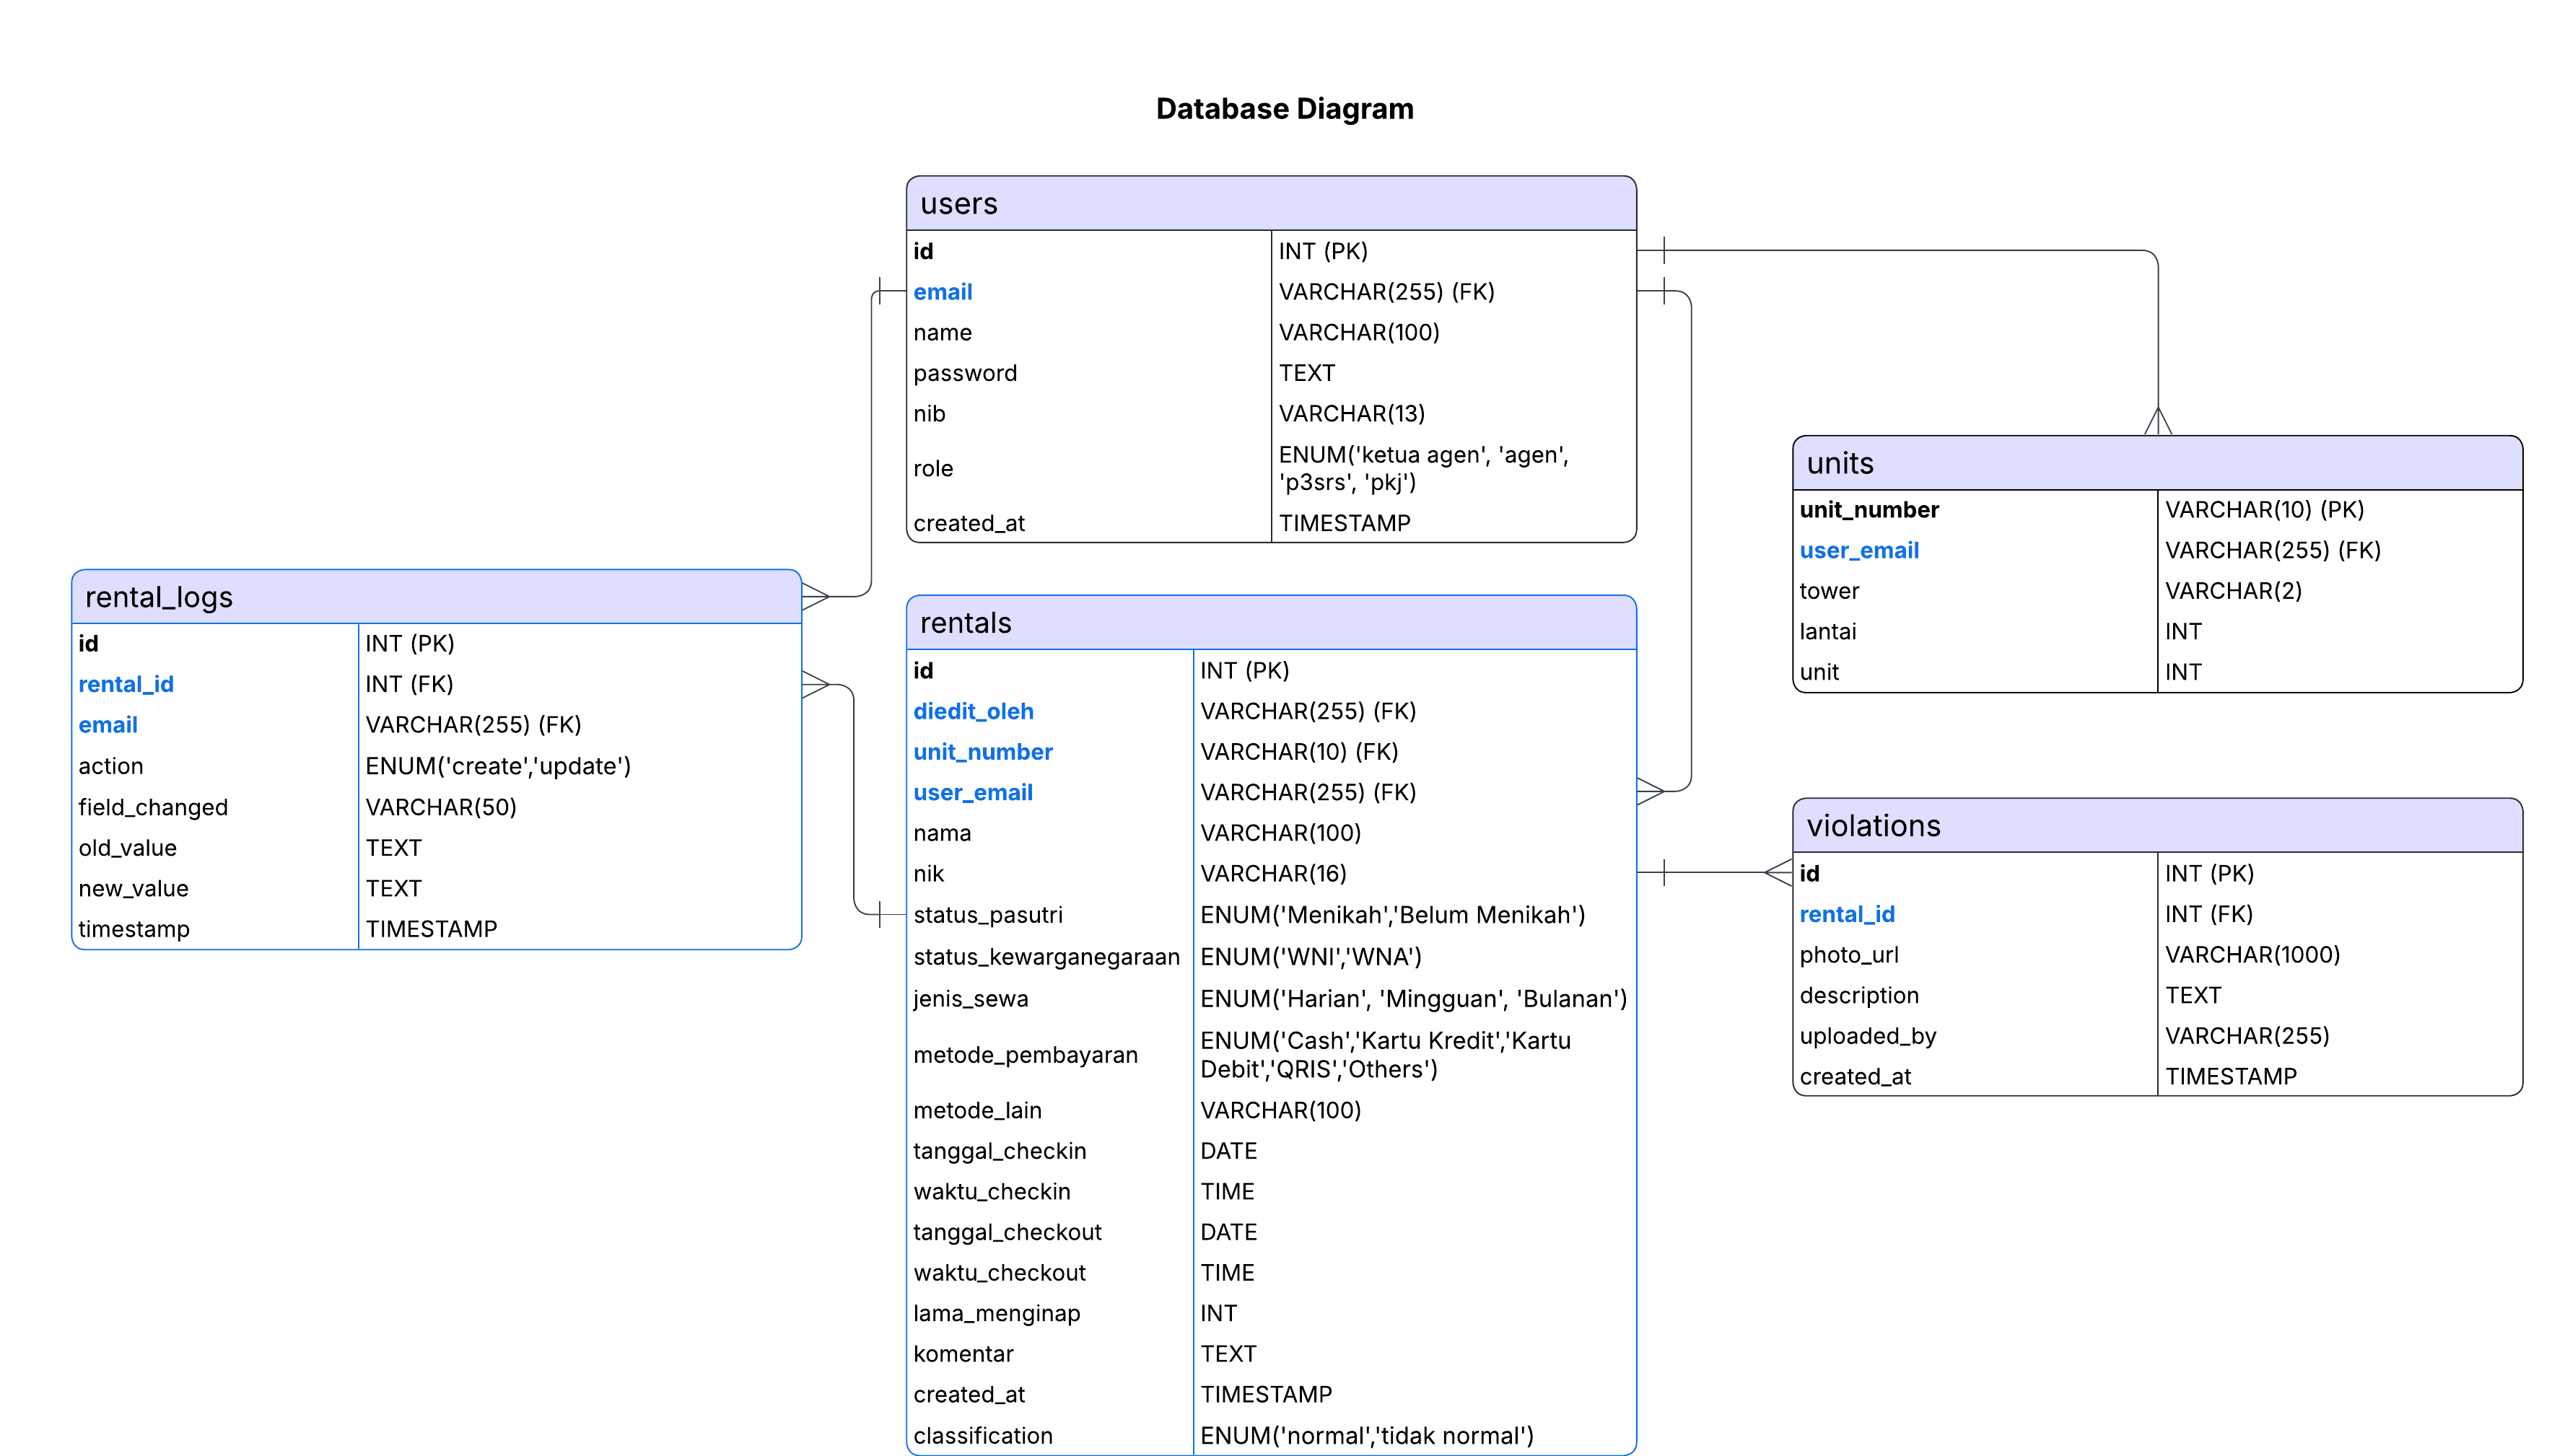
\includegraphics[width=0.7\textwidth, height=0.6\textheight, keepaspectratio]{Gambar/Database Diagram Sebelum.png}
        \caption{Database Diagram Sistem (Sebelum Integrasi)}
        \label{fig:db_diagram_sebelum}
    \end{figure}
    Gambar~\ref{fig:db_diagram_sebelum} menunjukkan struktur fisik kelima tabel tersebut pada basis data lokal sebelum disatukan dengan ekosistem SRusun. Skema ini berfokus utama pada fungsionalitas \textit{login} mandiri melalui tabel \texttt{users} serta pengelolaan siklus penyewaan dasar melalui tabel \texttt{rentals}, \texttt{units}, \texttt{rental\_logs}, dan \texttt{violations}.
\end{enumerate}

\subsubsection{Fase Setelah Integrasi (Ekosistem Terpusat)}
Fase ini membawa perubahan signifikan pada arsitektur otorisasi. Pengguna yang mengakses tautan \url{https://visitor.thejarrdin.com/} akan secara otomatis dialihkan ke halaman \textit{login} aplikasi \textit{Member} The Jarrdin. Proses pendaftaran dan \textit{login} mandiri ditiadakan, digantikan oleh mekanisme \textit{Single Sign-On} (SSO) menggunakan token JWT (JSON \textit{Web Token}) dari basis data utama SRusun. 

\begin{enumerate}
    % \item \textbf{Arsitektur dan Alur Kerja Sistem (\textit{Flowchart})} \\
    % Setelah autentikasi SSO berhasil, pengguna dapat mengakses sistem \textit{data capture} ini melalui menu terintegrasi bernama ``Penyewaan Unit''. Alur ini menjadikan operasional jauh lebih ringkas karena sistem langsung mengenali identitas dan peran pengguna dari aplikasi induk tanpa memerlukan autentikasi ganda.

    % \begin{figure}[H]
    %     \centering
    %     \includegraphics[width=0.7\textwidth]{Gambar/Flowchart Sistem Data Capture Sesudah.png}
    %     \caption{Flowchart untuk Sistem \textit{Data Capture} (Setelah Integrasi)}
    %     \label{fig:flowchart_data_capture_sesudah}
    % \end{figure}
    % Gambar~\ref{fig:flowchart_data_capture_sesudah} mengilustrasikan alur operasional yang lebih ringkas. Pelaku Komersil tidak lagi perlu melakukan pendaftaran terpisah, melainkan hanya perlu melakukan {login} melalui aplikasi induk {Member} The Jarrdin. Setelah itu, pengguna langsung diarahkan ke layar {dashboard} terpersonalisasi dan dapat mengakses seluruh fitur {data capture} melalui menu "Penyewaan Unit".
    
    \begin{figure}[H]
        \centering
        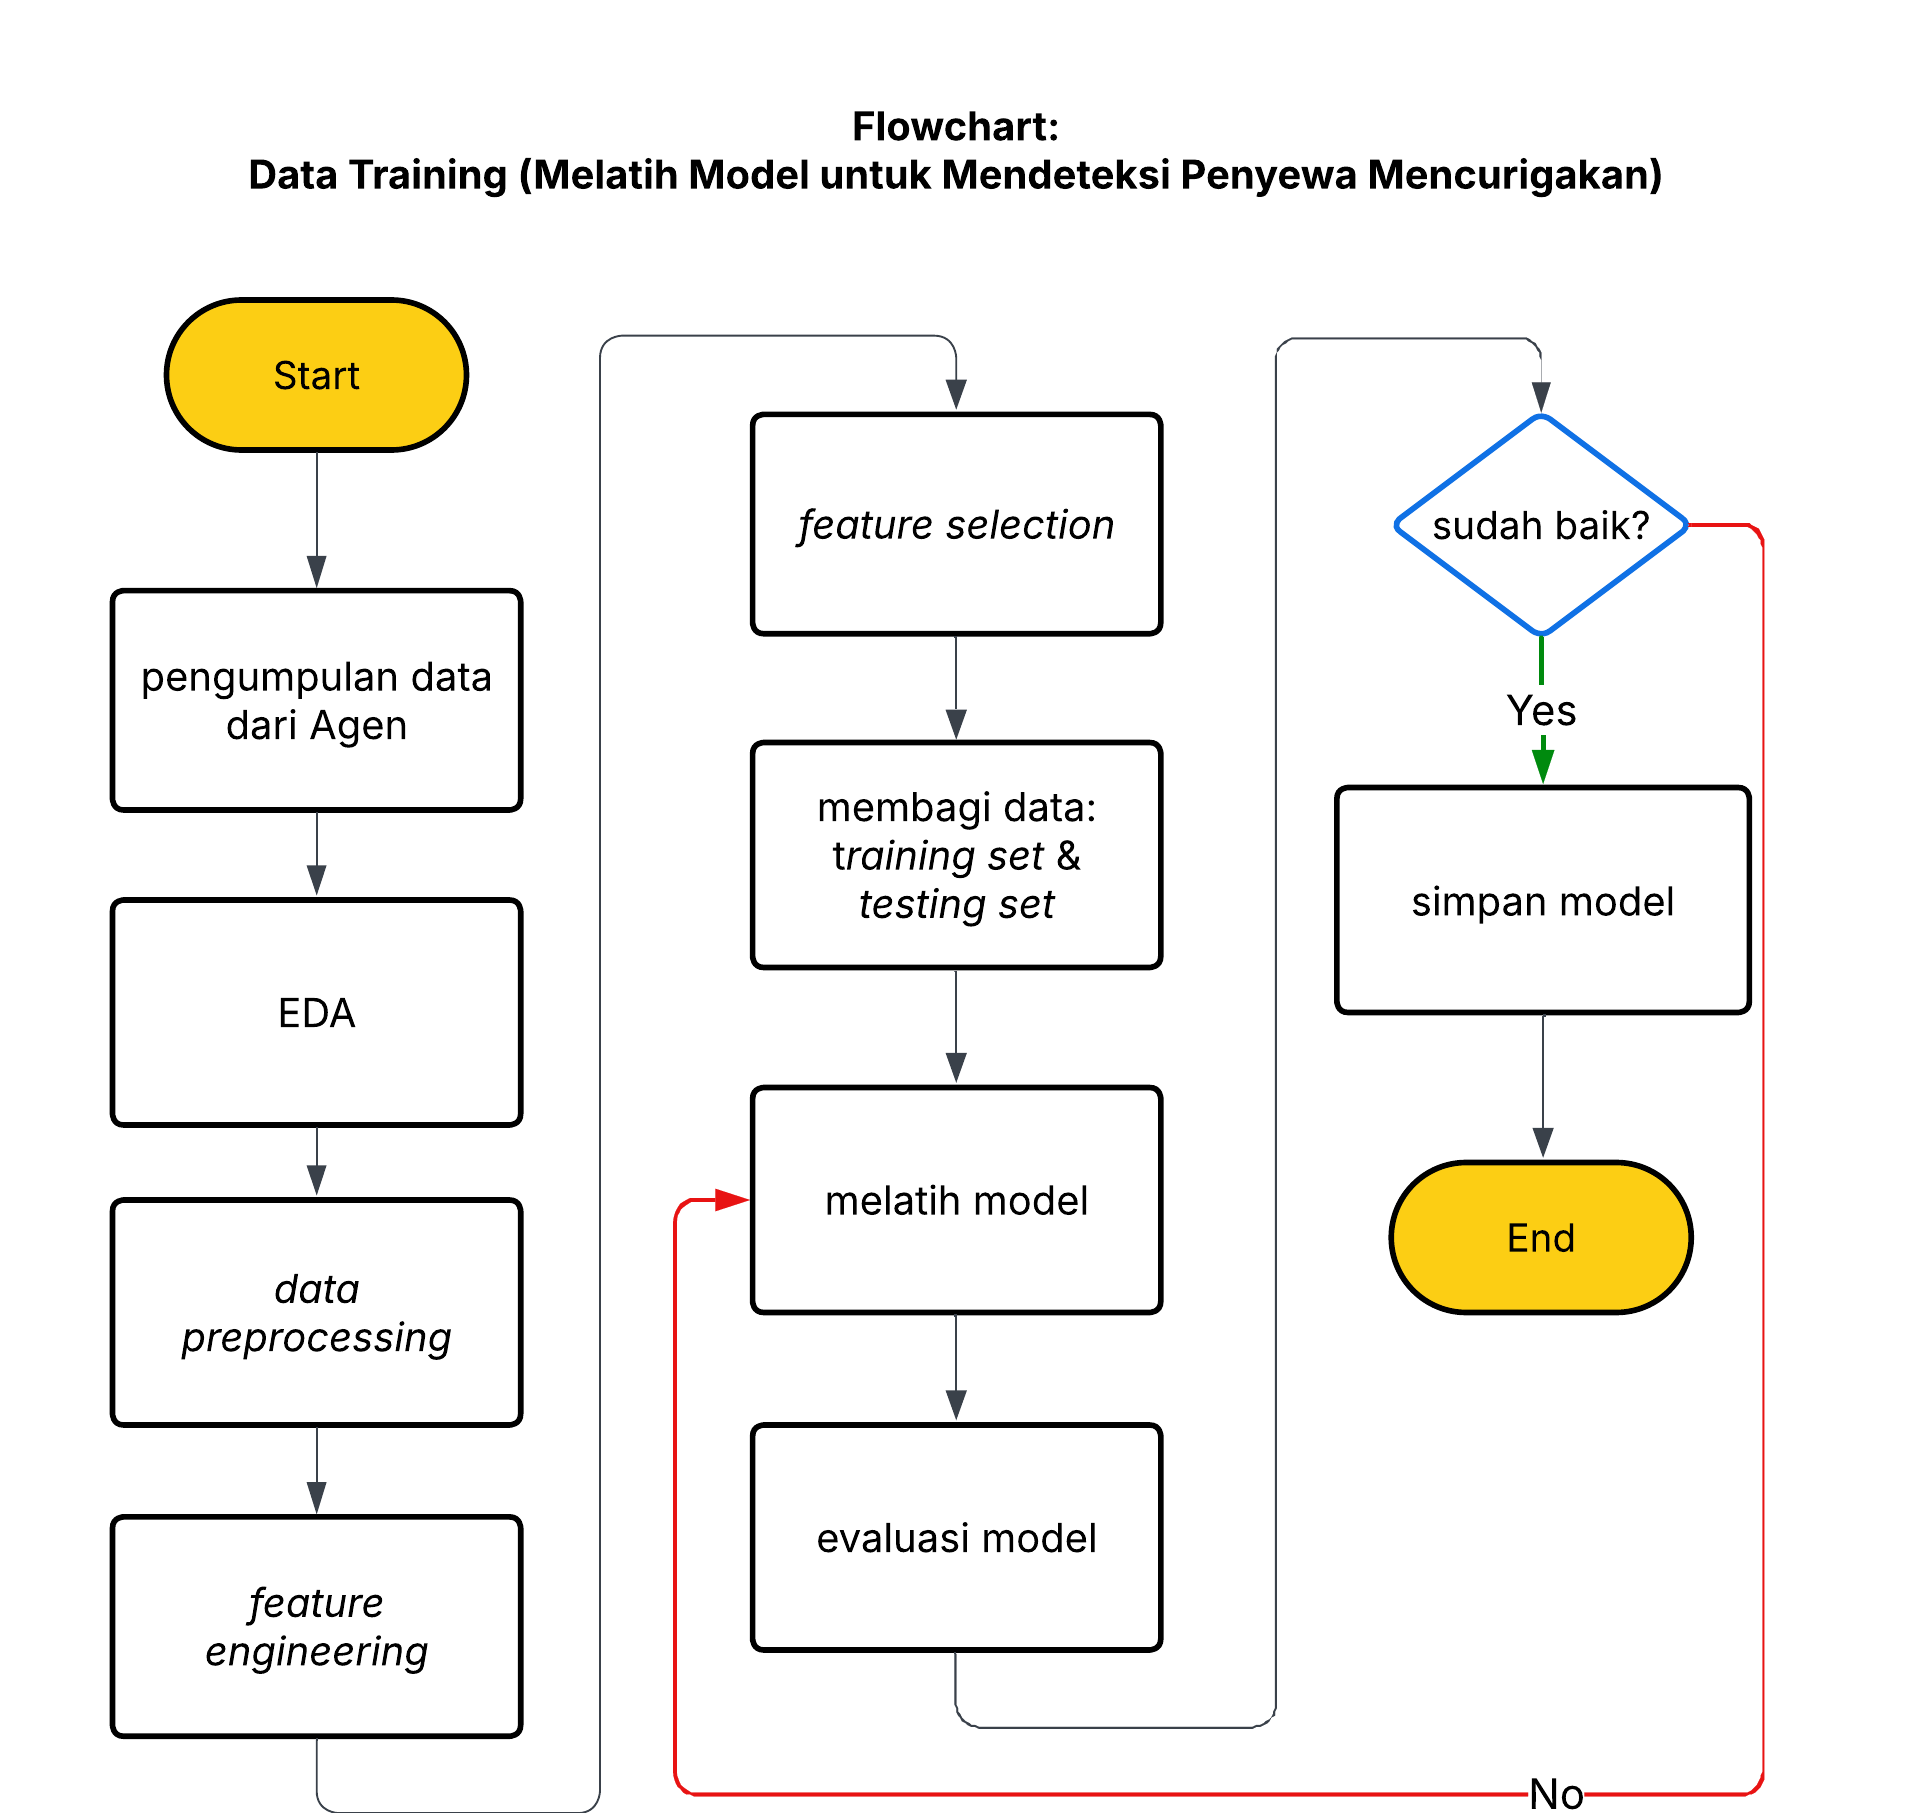
\includegraphics[width=0.7\textwidth]{Gambar/Flowchart Proses Data Training.png}
        \caption{Flowchart \textit{Data Training} (Sistem Terintegrasi)}
        \label{fig:flowchart_data_training}
    \end{figure}
    Gambar~\ref{fig:flowchart_data_training} menunjukkan proses lanjutan setelah data terkumpul secara terpusat. Data historis penyewa melalui tahap pra-pemrosesan untuk digunakan sebagai data pelatihan (\textit{training data}) bagi model klasifikasi \textit{machine learning}.

    \begin{figure}[H]
        \centering
        
\includegraphics[width=0.7\textwidth]{Gambar/Flowchart Proses Analisis & Notif.png}
        \caption{Flowchart untuk Deteksi Penyewa Mencurigakan}
        \label{fig:flowchart_deteksi_penyewa_mencurigakan}
    \end{figure}
    Gambar~\ref{fig:flowchart_deteksi_penyewa_mencurigakan} menggambarkan mekanisme inferensi model. Data penyewa baru yang diinputkan akan dianalisis oleh algoritma. Jika sistem mendeteksi keberadaan parameter yang mencurigakan (misalnya metode pembayaran tidak biasa, waktu \textit{check-in} tidak wajar, atau durasi inap sangat singkat), maka sistem secara otomatis memberikan notifikasi peringatan dini kepada pihak pengelola melalui \textit{dashboard}.

    \item \textbf{Interaksi Pengguna (\textit{Use Case Diagram})}
    \begin{figure}[H]
        \centering
        \includegraphics[width=0.47\textwidth, height=0.6\textheight, keepaspectratio]{Gambar/Use Case Diagram System Sesudah.png}
        \caption{\textit{Use Case Diagram} Sistem Terintegrasi}
        \label{fig:use_case_setelah}
    \end{figure}
    Berdasarkan Gambar~\ref{fig:use_case_setelah}, alur operasional sistem menjadi lebih ringkas karena aktor dan hak aksesnya kini diwariskan secara langsung dari sistem aplikasi induk {Member} The Jarrdin. Pelaku Komersil tidak lagi perlu melakukan pendaftaran terpisah, melainkan hanya perlu melakukan \textit{login} melalui aplikasi induk tersebut. Setelah berhasil {login}, pengguna langsung diarahkan ke layar {dashboard} terpersonalisasi dan dapat mengakses seluruh fitur {data capture} melalui menu ``Penyewaan Unit''. Dalam ekosistem yang terintegrasi ini, Pelaku Komersil hanya memiliki akses untuk mengelola data unit miliknya sendiri. Di sisi lain, Pengelola (Ketua Agen, P3SRS, atau PKJ) diberikan kewenangan administratif yang lebih luas untuk melihat rekapitulasi data dari seluruh pelaku komersil, mengelola {master} unit, serta meninjau laporan pelanggaran.

    \item \textbf{Struktur Basis Data (ERD dan \textit{Database Diagram})}
    \begin{figure}[H]
        \centering
        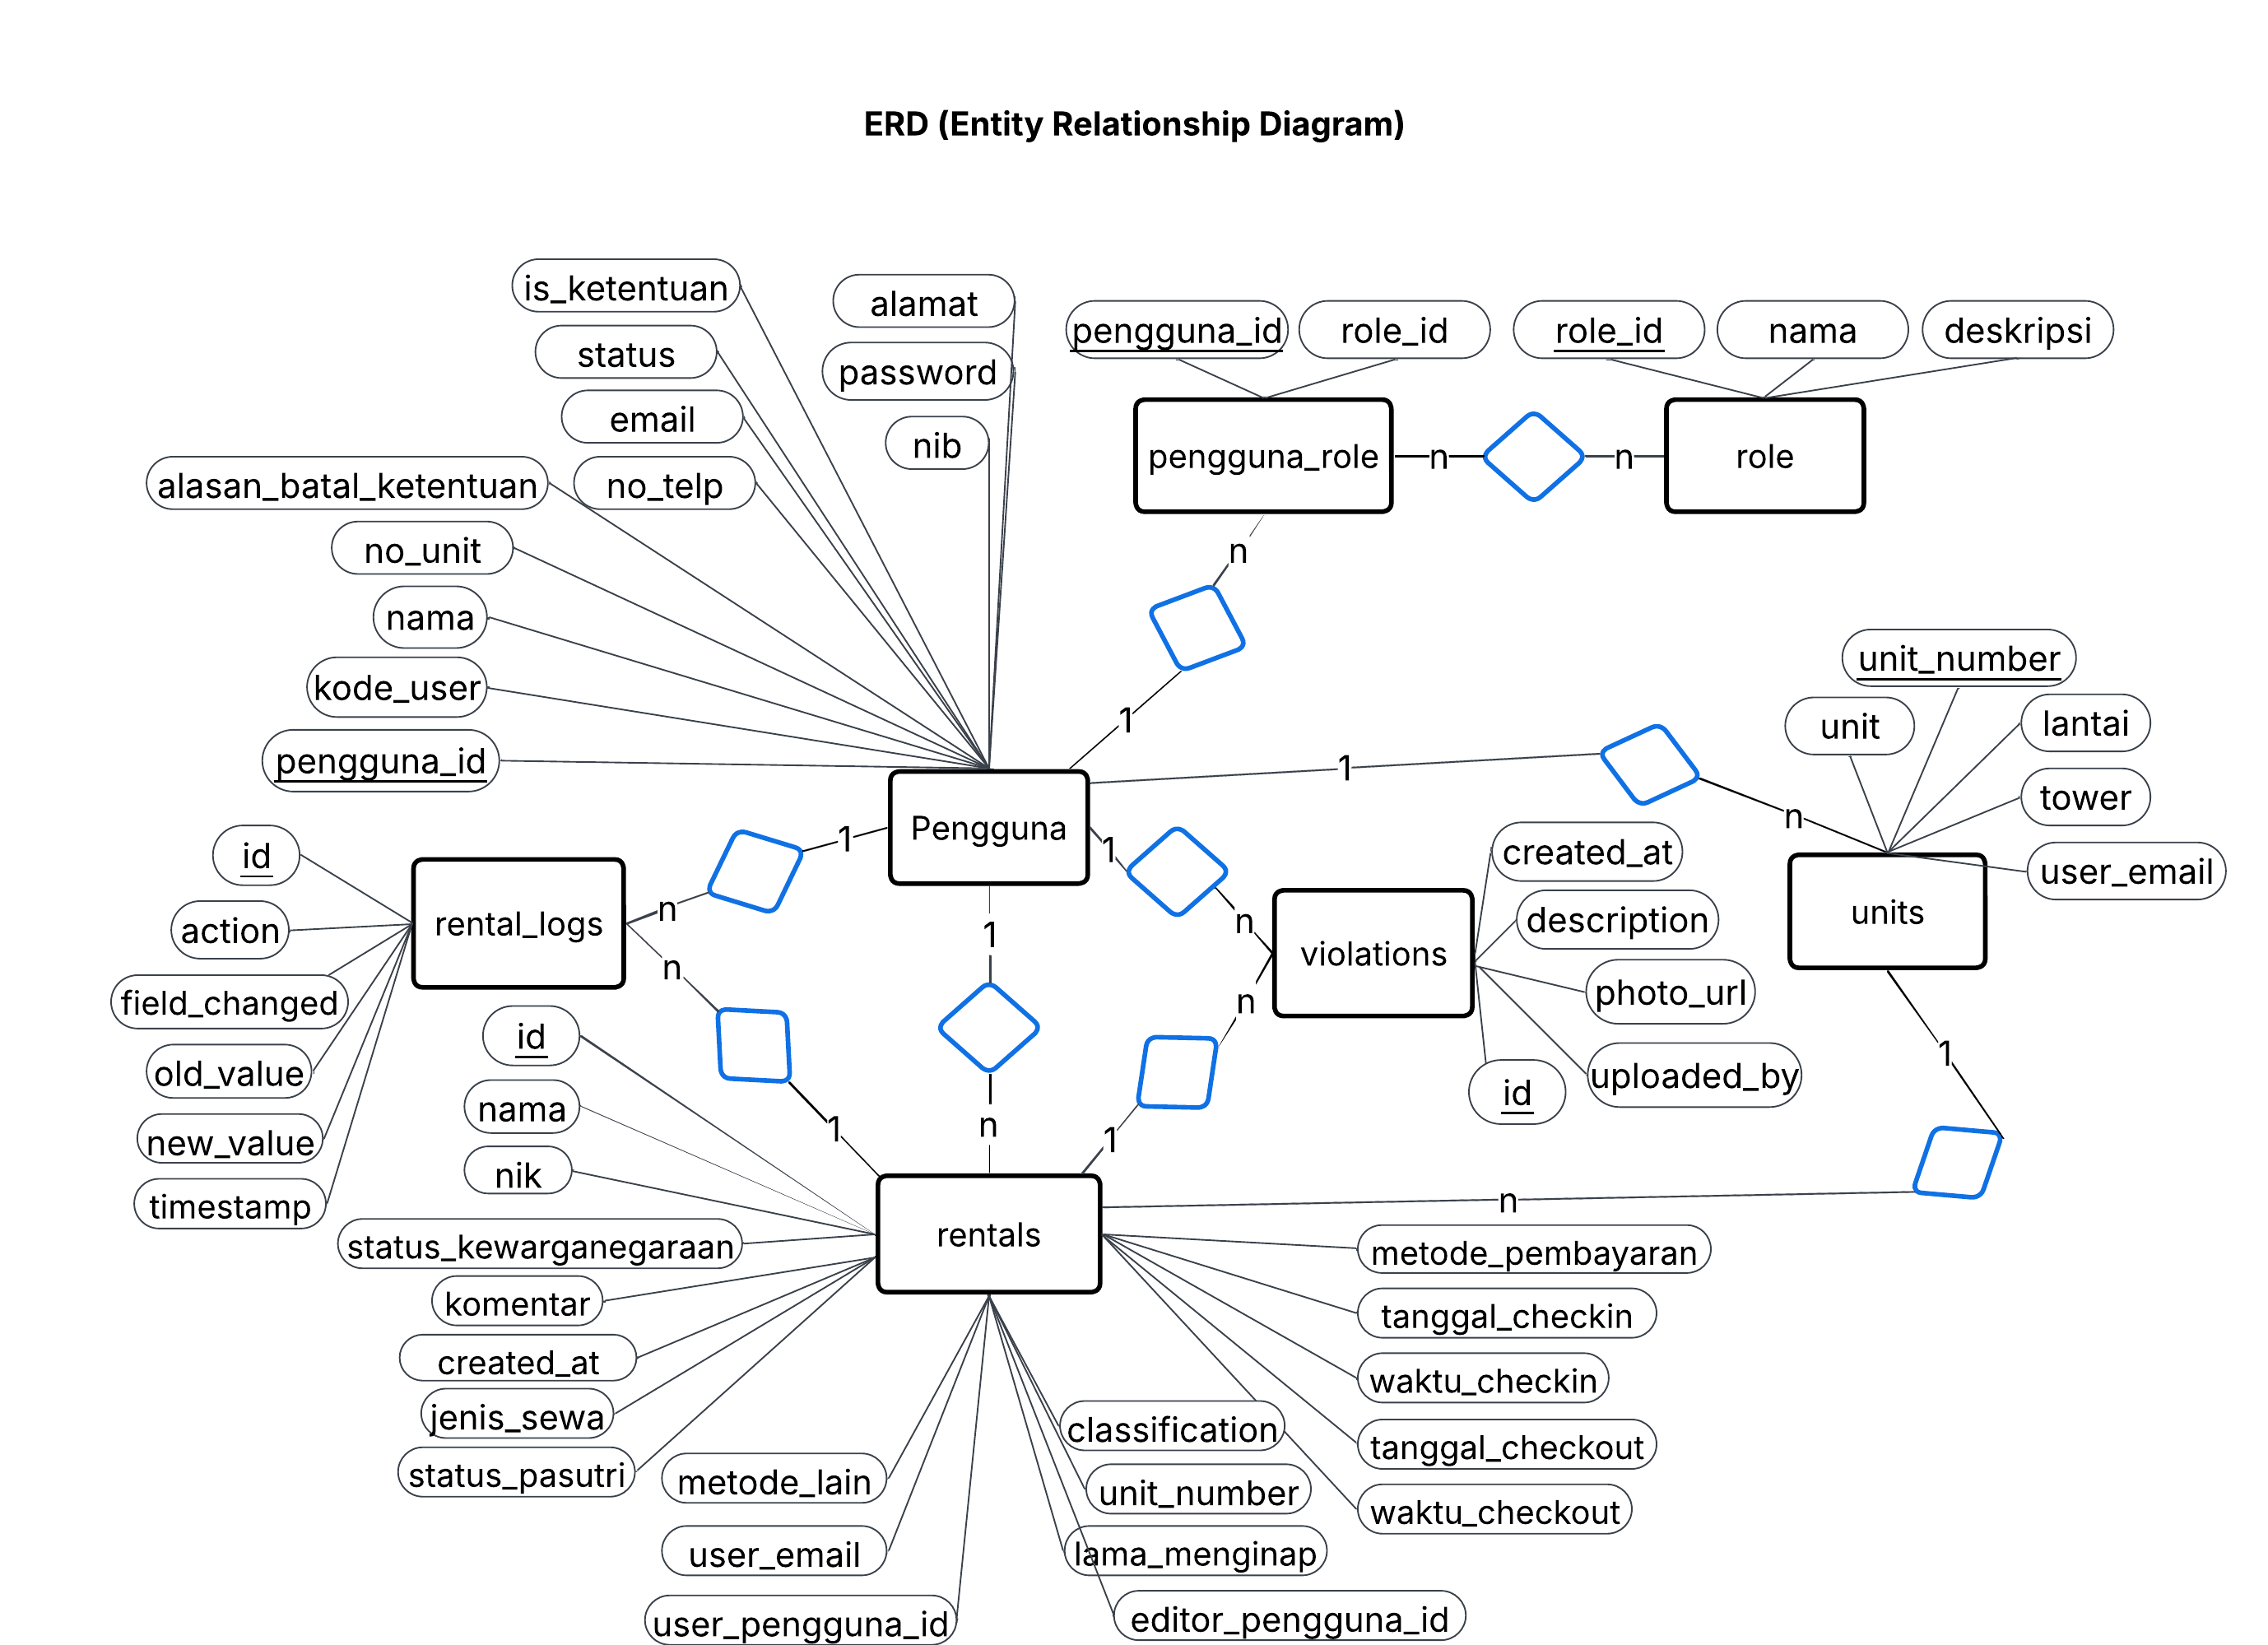
\includegraphics[width=0.8\textwidth]{Gambar/ERD Sesudah.png}
        \caption{Entity Relationship Diagram (ERD) Sistem Terintegrasi}
        \label{fig:erd_setelah}
    \end{figure}
    Struktur basis data (Gambar~\ref{fig:erd_setelah}) mengalami penyesuaian untuk mendukung sentralisasi. Tabel \texttt{users} lokal dihapus dan digantikan oleh tabel \texttt{pengguna}, \texttt{role}, dan \texttt{pengguna\_role} yang dikelola secara terpusat oleh basis data SRusun. Relasi tabel \texttt{rentals} (data penyewa), \texttt{units} (data kamar), \texttt{violations} (data pelanggaran visual), dan \texttt{rental\_logs} (riwayat perubahan) dikaitkan menggunakan kunci tamu (\textit{foreign key}) berupa \texttt{user\_email} yang merujuk pada identitas pengguna di sistem induk.

    \begin{figure}[H]
        \centering
        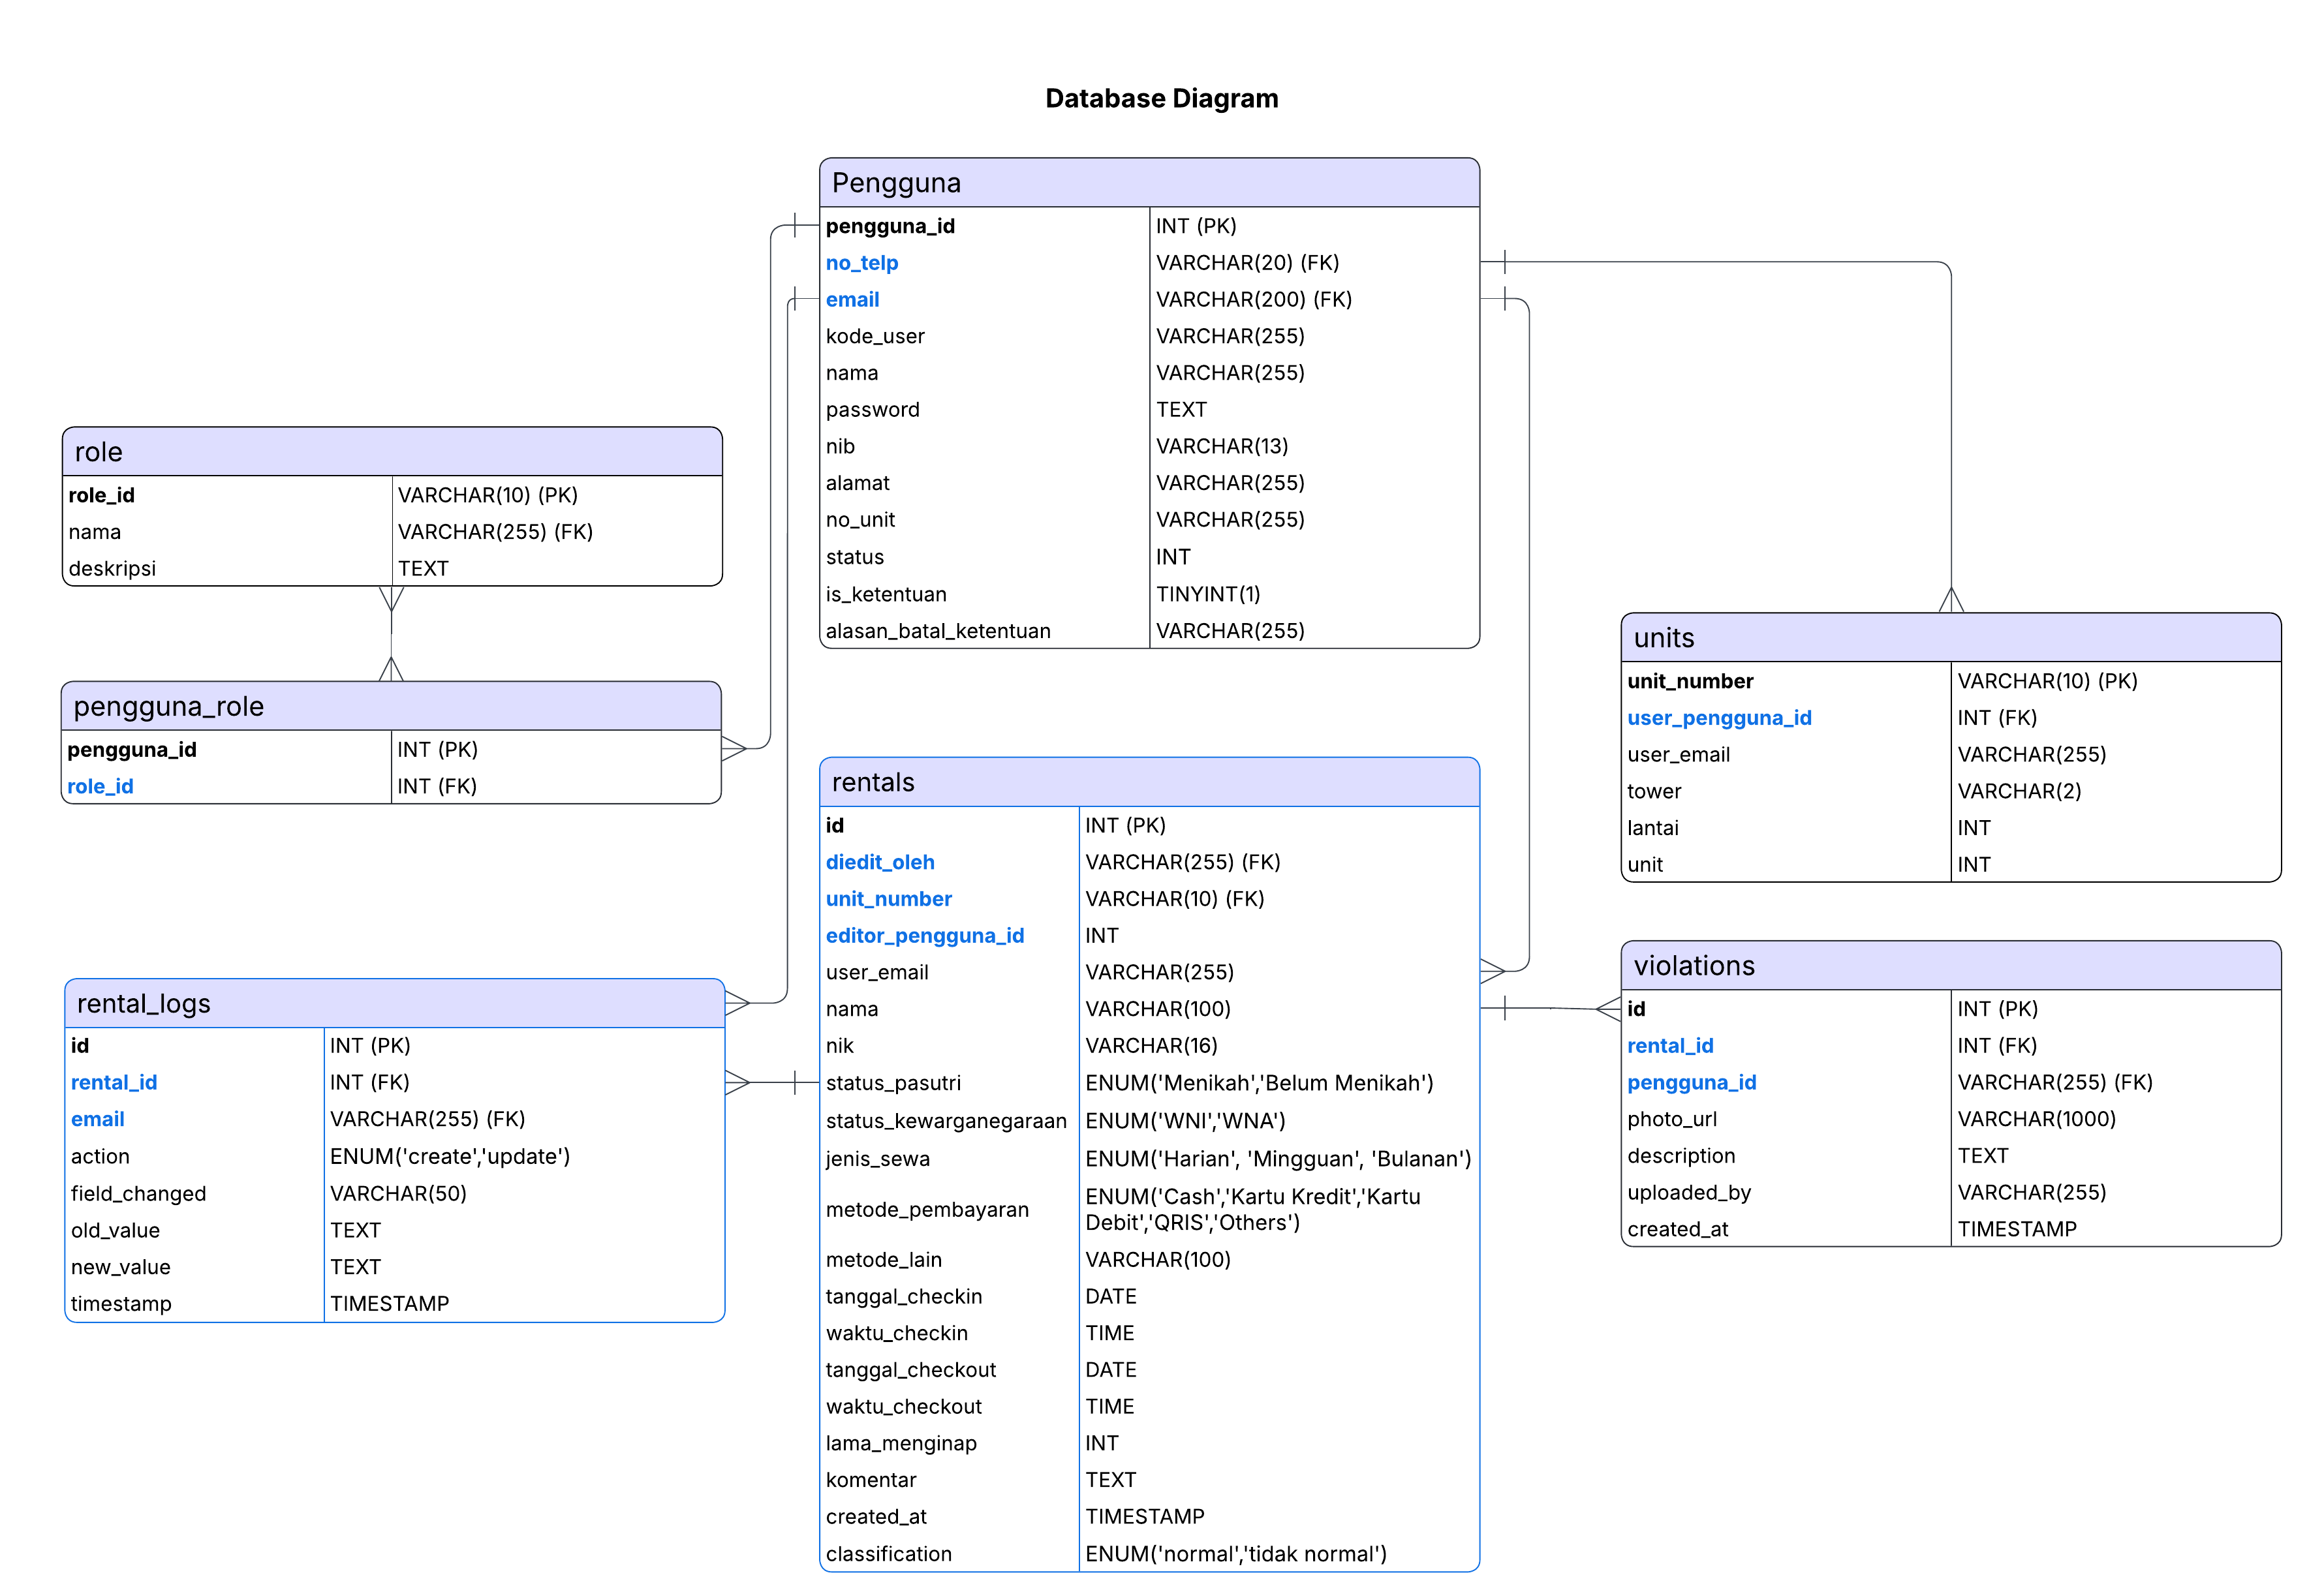
\includegraphics[width=0.7\textwidth, height=0.6\textheight, keepaspectratio]{Gambar/Database Diagram Sesudah.png}
        \caption{Database Diagram Sistem Terintegrasi}
        \label{fig:db_diagram_setelah}
    \end{figure}
    Gambar~\ref{fig:db_diagram_setelah} memperlihatkan skema fisik (\textit{physical data model}) dari tabel-tabel di dalam sistem basis data MySQL setelah proses integrasi selesai. Desain skema ini telah dioptimalkan untuk memastikan integritas data terpusat, mendukung penyimpanan data kualitatif pelanggaran, menjamin pencatatan \textit{audit log}, serta memfasilitasi ekstraksi data yang efisien untuk keperluan pelatihan model \textit{machine learning}.
\end{enumerate}






















































\subsection{Fitur Utama dan Implementasi Logika Bisnis}
Sistem yang dibangun memiliki fitur-fitur krusial yang saling terintegrasi untuk mendukung operasional pengelolaan hunian.

\subsubsection{1. Input Data Terstandarisasi dan Validasi}
Formulir input dirancang untuk menangkap variabel-variabel penting guna keperluan analisis profil penyewa. Data yang dicatat meliputi Nomor Induk Kependudukan (NIK), status pernikahan (Menikah/Belum Menikah), kewarganegaraan, unit menginap, serta rincian sewa seperti tanggal \textit{check-in/check-out}.
\begin{itemize}
    \item \textbf{Kalkulasi otomatis}: sistem secara otomatis menghitung durasi lama menginap berdasarkan selisih tanggal masuk dan keluar.
    \item \textbf{Validasi NIB}: sistem secara otomatis cek apakah NIB valid.
    \item \textbf{Validasi email dan password}: sistem secara otomatis cek apakah email dan password user valid.
\end{itemize}

\subsubsection{2. Log Riwayat Perubahan (\textit{Audit Trail})}
Fitur keamanan data yang paling krusial adalah \textit{Log History}. Sistem merekam setiap aktivitas perubahan data secara rinci (\textit{create, update}). Mekanisme ini bekerja dengan cara sebagai berikut.
\begin{itemize}
    \item Mencatat identitas pengubah (berdasarkan email), waktu perubahan (\textit{timestamp}), serta membandingkan nilai lama (\textit{old value}) dengan nilai baru (\textit{new value}).
    \item Log ini bersifat permanen dan dapat diunduh dalam format CSV untuk keperluan audit investigasi apabila terjadi sengketa data.
\end{itemize}

\begin{figure}[H]
    \centering
    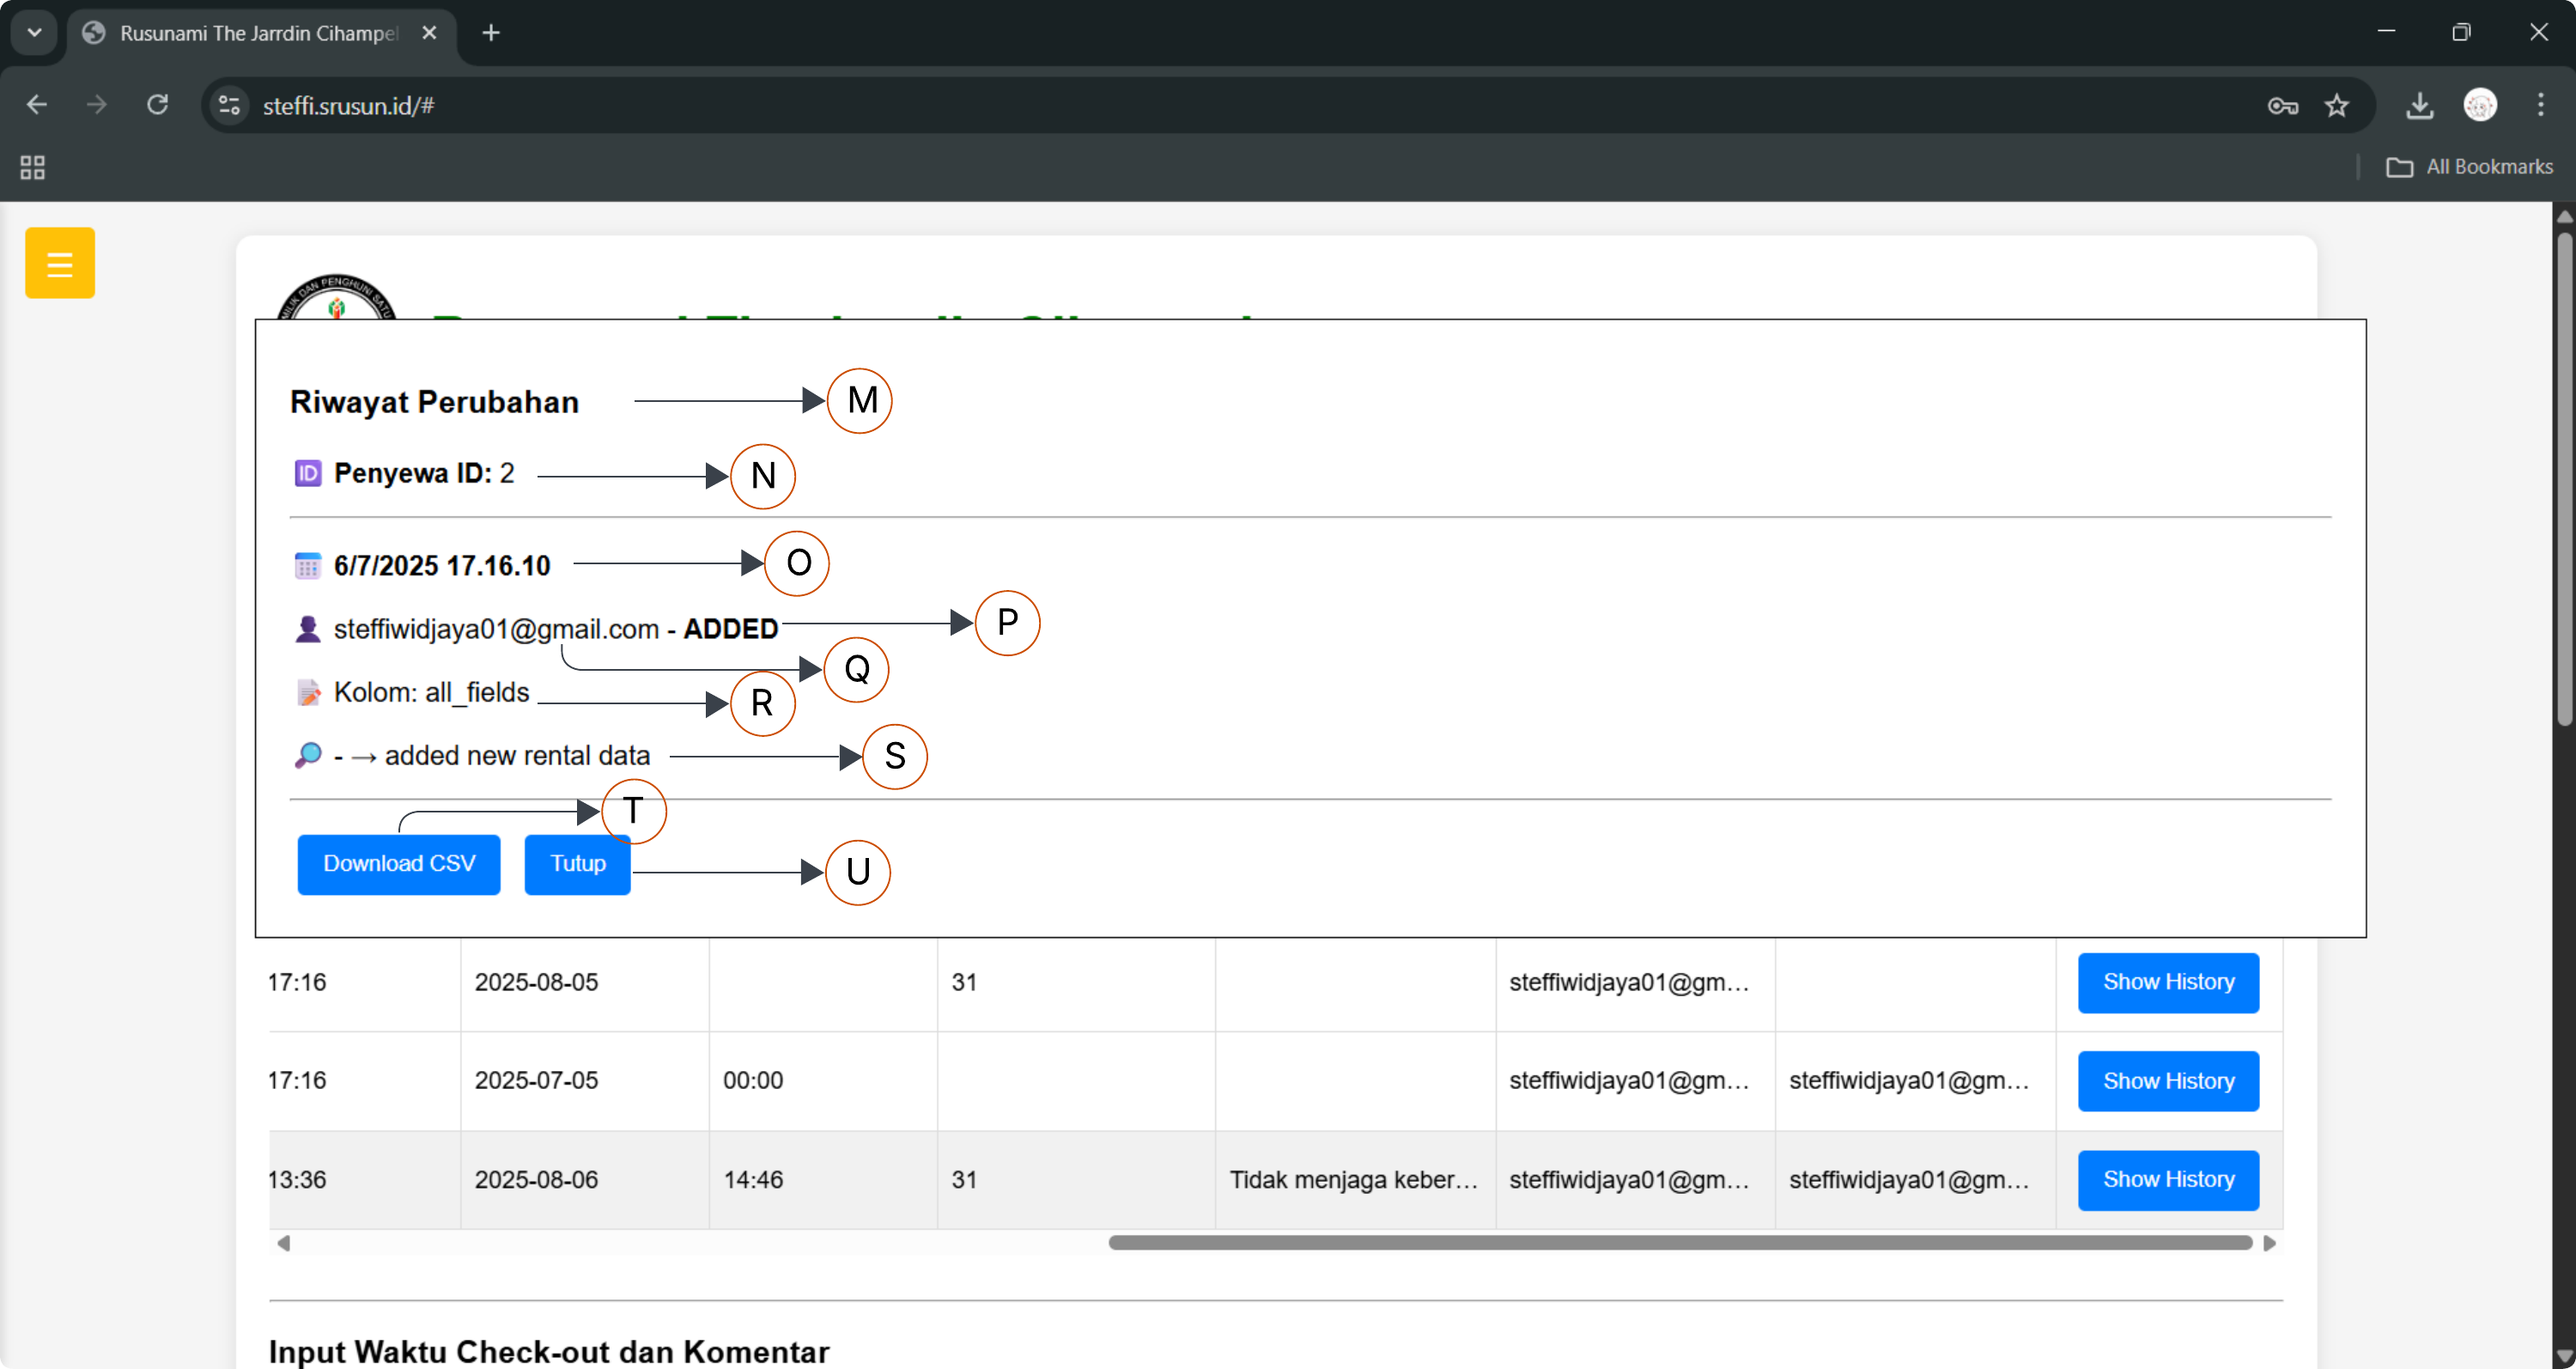
\includegraphics[width=0.7\textwidth]{Gambar/halaman lih 3 js.png}
    \caption{Tampilan Detail Riwayat Perubahan Data}
    \label{fig:log_history}
\end{figure}

\subsubsection{3. Manajemen Unit dan Status Okupansi}
Sistem memiliki logika untuk memantau ketersediaan unit secara \textit{real-time}.
\begin{itemize}
    \item \textbf{Deteksi status}\\
    Status unit (\textit{Occupied/Available}) ditentukan berdasarkan tanggal \textit{checkout}. Jika tanggal \textit{checkout} unit tersebut masih di masa depan dibandingkan tanggal hari ini, unit otomatis ditandai sebagai terisi.
    \item \textbf{Manajemen admin}\\
    Pengguna dengan peran Pengelola memiliki hak akses penuh untuk menambah, mengubah, atau menghapus data unit master, serta melihat performa okupansi per Pelaku Komersil.
\end{itemize}

\subsubsection{4. Visualisasi Dashboard Statistik}
Untuk memudahkan pengambilan keputusan, sistem menyediakan \textit{dashboard} visual yang menyajikan data statistik sebagai berikut.
\begin{itemize}
    \item \textbf{Grafik tren sewa}\\
    Menampilkan jumlah penyewaan harian atau bulanan menggunakan diagram garis.
    \item \textbf{Unit populer}\\
    Menampilkan unit-unit yang paling sering disewa menggunakan histogram, yang berguna untuk analisis preferensi penyewa.
    \item \textbf{Performa Pelaku Komersil}\\
    Khusus untuk Pengelola tersedia statistik untuk memantau produktivitas setiap Pelaku Komersil berdasarkan jumlah unit yang berhasil disewakan.
\end{itemize}

\subsubsection{5. Pelaporan Pelanggaran dengan Bukti Visual}
Fitur ini memungkinkan Pelaku Komersil atau Pengelola untuk mencatat pelanggaran yang dilakukan penyewa.
\begin{itemize}
    \item \textbf{Bukti digital}\\
    Pelapor dapat mengunggah bukti foto yang relevan (misalnya kerusakan aset atau temuan barang terlarang).
    \item \textbf{Kategori pelanggaran}\\
    Sistem menyediakan daftar kategori pelanggaran baku (seperti kebisingan, asusila, atau kerusakan fasilitas) untuk standarisasi laporan.
\end{itemize}

\subsubsection{6. Ekspor Data Laporan}
Untuk kebutuhan arsip dan analisis eksternal, sistem menyediakan fitur unduh data dalam format \textbf{.CSV}. Laporan yang dapat diunduh meliputi:
\begin{itemize}
    \item aata lengkap seluruh penyewa,
    \item log aktivitas sistem secara keseluruhan, dan
    \item log spesifik riwayat perubahan data untuk satu penyewa tertentu.
\end{itemize}